\chapter{Angular Momenta Algebra}
\section{One angular momentum}
Soit $\vec j$, un moment angulaire générique. Pour peut l'écrire sous la forme de deux 
opérateurs.
\begin{equation}
\left\{ \begin{array}{l}
{\bf j}^2 \; \vert j m \rangle  =  \hbar^2 j(j + 1) \vert j m \rangle \\
j_{z} \; \vert j m \rangle  =  \hbar m  \; \vert j m \rangle  
 \end{array} \right.
\end{equation}
où $m = j, (j-1), \ldots, -j $ est la valeur propre de $j_z$, c'est-à-dire la projection sur un axe privilégié.
Si on détermine $j_z$ et $\vec j^2$, il nous sera impossible de définir en même temps
$j_y$ et $j_x$ (principe d'incertitude et non-commutation).\\

Quel est l'impact de la symétrie ? Si l'on prend des $\ket{jm}$ sur lequel on applique un opérateur
de rotation $D(\omega)$, qu'est ce qui se passe ? 
Il va être transformé, mais on retrouve une somme finie limitée aux états de projections $m'$ en restant sur le même $j$ donné. 
\begin{equation}
D(\omega)  \vert j m \rangle  =  
\sum_{m'}
\vert j m' \rangle
\underbrace{
\langle jm' \vert  D(\omega) \vert j m \rangle}
_{ {\cal  D}^j_{m'm} (\omega) }
\end{equation}
où $\omega$ est la triade des angles d'\textsc{Euler} : c'est une séquence de trois rotation qui permet
 de passer d'un repère à un autre. Une rotation de $\alpha$ autour de $z$ s'écrit
\begin{equation}
R_z(\alpha) = \exp\left(-i\frac{\alpha j_z}{\hbar}\right)
\end{equation}
On comprend alors que $D(\omega)$ n'est qu'une séquence de trois opérateurs de rotation mais pas
n'importe laquelle : selon les angles d'\textsc{Euler}. Cet opérateur nous permet d'envisager 
n'importe quelle rotation de systèmes d'axes et nous informe comment le $\ket{jm}$ s'est 
transformé.\\

Intéressons-nous à l'élément matriciel suivant
\begin{equation}
\underbrace{
\langle jm' \vert  D(\omega) \vert j m \rangle}
_{ {\cal  D}^j_{m'm} (\omega) }
\end{equation}
C'est l'élément matriciel de l'opérateur rotation entre deux vecteurs d'états $\ket{jm}$ et
$\ket{jm'}$, mais on reste dans l'espace $2j+1$. C'est la \textbf{représentation matricielle} de
dimension $2j+1$ où $\omega$ donne la triade des angles d'\textsc{Euler} : nous avons fait apparaitre
la dimension du groupe de rotation.
\begin{equation}
D(\omega)\ket{jm} = \sum_i \ket{i}\bra{i} D(\omega)\ket{jm}
\end{equation}
Nous pouvons sommer sur $j'm'$
\begin{equation}
\sum_{j’m’} \ket{j’m’}\underbrace{\bra{j’m’} D(\omega)\ket{jm}}_{\delta_{jj’}}
\end{equation}
On remarque que cette matrice est identique : on peut raisonner pour une valeur de $j$. Il s'agit
d'une représentation matricielle diagonale car, dans le groupe de rotation, on va mélanger les
fonctions au sein d'un même sous-espace mais on ne mélange pas les $j$ différents. Dans cette
base la, les opérateurs de rotation ont la propriété géniale de ne pas mélanger les $j$. C'est
\textbf{irréductible}, il n'y a pas espoir d'aller au delà de ce symbole de Kronecker.\\

On note ${\cal  D}^j_{m'm} (\omega)$ l'ensemble ces matrices. Lorsqu'on écrit un $\ket{jm}$, 
il va se comporter par rapport à l'opérateur de rotation en accord avec les représentation
du groupe $SO3$. Si $j=0$, c'est la \textit{représentation triviale} qui correspond, dans 
$SO3$, à l'orbitale $s$ (la boule). C'est $Y_0^0$ qui est indépendant de $\theta,\phi$ que
l'on peut tourner comme on veut. Si $j=1$, ce sont les trois fonctions derrière une orbitale
$p$ ($Y^1_1,Y^1_0,Y^1_{-1}$) que l'on appelle $\cal{D}^1$. $\cal{D}^3$ c'est $F$, etc. Derrière
une fonction propre de $\vec j^2$ et $j_z$, il existe une infinité de matrices de rotation.\\

On peut passer d'une valeur de $m$ à une autre avec les opérateurs élévateurs et abaisseurs
\begin{equation}
j_{\pm} \; \vert j m \rangle  =  
\hbar 
[ j(j+1) - m(m \pm 1) ]^{1/2}  
\; \vert j (m \pm 1) \rangle
\end{equation}


\section{Coupling of two  angular momenta}
Nous avons ici deux moments angulaires qui peuvent provenir de deux particules différentes ou
d'une seule avec deux moments angulaires (spin et orbite). En mécanique quantique, c'est assez
simple à écrire : on l'écrit sous la forme d'un \textit{ket}, et lorsque l'on écrit un nombre
quantique dans ce \textit{ket} nous retrouvons une équation aux valeurs propres. Il faut chaque
fois se dire \textit{quelle est l'équation aux valeurs propres}
\begin{equation}
\left\{ \begin{array}{l}
{\bf j}_1^2 \; \vert j_1 m_1 \rangle  =  \hbar^2 j_1(j_1 + 1) \vert j_1 m_1 \rangle \\
j_{1z} \; \vert j_1 m_1 \rangle  =  \hbar m_1 \;\vert j_1 m_1 \rangle  
 \end{array} \right.
\end{equation}
où $m_1 = j_1, (j_1-1), \ldots, -j_1$. On peut faire de même pour le second moment angulaire
\begin{equation}
\left\{ \begin{array}{l}
{\bf j}_2^2 \; \vert j_2 m_2 \rangle  =  \hbar^2 j_2(j_2 + 1) \vert j_2 m_2 \rangle \\
j_{2z} \; \vert j_2 m_2 \rangle  =  \hbar m_2 \;\vert j_2 m_2 \rangle  
 \end{array} \right.
\end{equation}
où $m_2 = j_2, (j_2-1), \ldots, -j_2$. Si on veut mettre ensemble ces deux moments angulaires, 
nous allons faire apparaître les produits suivants
\begin{equation}
\vert j_1 m_1 j_2 m_2  \rangle \equiv 
\vert j_1 m_1 \rangle \vert j_2 m_2 \rangle 
= \vert j_2 m_2 \rangle  \vert j_1 m_1 \rangle
\end{equation}
On peut voir ça comme des fonctions propres. On peut définir un \textsc{ecoc} car elles commutent
entre-elles (mais pas avec l'hamiltonien)
\begin{equation}
\mbox{ECOC}~ = \{ {\bf j}_1^2, j_{1z}, {\bf j}_2^2, j_{2z} \}
\end{equation}
Il s'agit de la \textbf{représentation découplée}.\\

On va pouvoir passer d'une représentation à une autre en effectuant un changement d'
\textsc{ecoc}. A partir de $\vec j_1$ et $\vec j_2$, construisons un moment angulaire
total.
\begin{equation}
{\bf j} = {\bf j}_1 + {\bf j}_2 \Rightarrow 
{\bf j}^2 = {\bf j}_1^2 + {\bf j}_2^2 + 2 \; {\bf j}_1  \cdot {\bf j}_2
\end{equation}
L'élévation au carré fait apparaître un terme de couplage entre ces deux moments angulaires. Si
nous restons dans une représentation découplée, il n'y a pas besoin d'invoquer ce terme de 
couplage. Par contre, il pourrait y avoir un terme qui force le couplage dans l'hamiltonien. Est-il
possible de construire un \textit{ket} avec trois moment angulaire et $m$, la projection du $j$ 
total sur l'axe $z$ ? Oui, c'est comme si nous avons quatre équations aux fonctions propres
\begin{equation}
\left\{ \begin{array}{l}
{\bf j}_1^2 \; \vert j_1 j_2 j m \rangle  =  \hbar^2 j_1(j_1 + 1) \vert j_1 j_2 j m \rangle \\
{\bf j}_2^2 \; \vert j_1 j_2 j m \rangle  =  \hbar^2 j_2(j_2 + 1) \vert j_1 j_2 j m \rangle \\
{\bf j}^2 \;  \vert j_1 j_2 j m \rangle  =  \hbar^2 j(j + 1)  \vert j_1 j_2 j m \rangle   \\
j_z \;  \vert j_1 j_2 j m \rangle  =  \hbar m  \vert j_1 j_2 j m \rangle   \\
 \end{array} \right.
\end{equation}
Avec cette fois-ci, comme \textsc{ecoc}
\begin{equation}
\mbox{ECOC}~ = \{ {\bf j}_1^2,  {\bf j}_2^2, {\bf j}^2, j_z \}
\end{equation}
Il s'agit de la \textbf{représentation couplée}.\\

La clef pour exprimer ce changement d'\textsc{ecoc} est d'exprimer l'un en fonction de l'autre. 
Pour cela, on va utiliser la relation de fermeture : on somme sur $m_1$ pour $j_1$ fixé et de 
même pour $m_2$
\begin{equation}
\vert j_1 j_2 j m \rangle = 
\sum_{m_1,m_2} \vert j_1 m_1 j_2 m_2 \rangle \langle 
j_1 m_1 j_2 m_2 
\vert j_1 j_2 j m \rangle 
\end{equation}
Le passage de l'un à l'autre donne un produit scalaire entre les deux. Ceci donnera la transformation
unitaire qui permet le changement d'\textsc{ecoc}. En connaissance ce coefficient, 
on pourra passer d'une représentation à l'autre : c'est un Clebsch-Gordan
\begin{equation}
\langle j_1 m_1 j_2 m_2 \vert j_1 j_2 j m \rangle= (-1)^{j_1 - j_2 + m} \sqrt{2j+1} \left(
\begin{array}{ccc}
j_1 & j_2 & j \\
m_1 & m_2 & -m 
\end{array} \right)
\end{equation}
Il ne sont pas facilement lisible car il y a pleins de façon différente de les lire. Mais la chose
à retenir, c'est que ce sont des $3j$ : tout ces coefficients sont reliés au symbole $3j$. Pourquoi
ce nom ? Car il y a trois moments angulaires : $j_1,j_2$ et la résultante. Tout ne sera pas permis
lorsque l'on couple des moments angulaires. Si nous avons $\vec j = \vec j1 + \vec j2$, la projection
sur $z$ donne $j_z=j_{1z}+j_{2z}$. Si $m$ est la projection sur $z$, il est évident que ceci implique
que $m=m_1+m_2$. Ceci est exprimé par la dernière ligne du coefficient de Clebsch-Gordan : la
somme doit être nulle. Il existe une seconde condition, venant de la quantification de $j$ :
l'addition vectorielle est quantifiée, toutes les possibilités de $j$ ne sont pas permises. D'où 
est ce que ceci vient ? Pas du ciel, mais à partir des opérateurs de montée et de descente.
\begin{equation}
\langle j_1 m_1 j_2 m_2 \vert j_1 j_2 j m \rangle \neq 0 ~\mbox{ssi }
\left\{
\begin{array}{l}
m = m_1 + m_2 \\
j = j_1 + j_2, j_1 + j_2 -1, \ldots, \vert j_1 - j_2 \vert
\end{array} \right.
\end{equation}
Dans cette base, on peut partitionner le groupe de rotation
\begin{equation}
{\cal D}^{(j_1)} \otimes {\cal D}^{(j_2)} = \sum_{\oplus j = |j_1-j_2|}^{j_1+j_2}\mathcal{D}^j=
{\cal D}^{(j_1+j_2)} \oplus  {\cal D}^{(j_1+j_2-1 )} \oplus
\ldots \oplus {\cal D}^{(\vert j_1-j_2 \vert)}
\end{equation}
Cette transformation bloc-diagonalise toute les matrices du bloc $SO3$ pour n'importe quel
angle de rotation (n'importe quel $\omega$). Toutes les $\mathcal{D}$ ne sont pas couplées car
elles possèdent des valeurs de $j$ différentes et les $j$ différents ne sont pas couplés. Nous
avons réduit une "grosse matrice" en une somme de sous-matrice.

\newpage
\exemple{couplage de deux électrons $p$.\\
Considérons deux électrons et oublions leurs spins : on couple les moments orbitaux
\begin{equation}
{\bf L} = {\bf l}_1 + {\bf l}_2
\longrightarrow L = l_1 + l_2, l_1 + l_2 -1, \ldots 
\vert l_1 - \l_2 \vert
\end{equation}
On en tire, avec les règles de quantification de l'addition vectorielle
\begin{equation}
{\bf L} = \vec{1} + \vec{1}
\longrightarrow L = 2,1,0
\end{equation}
\begin{center}
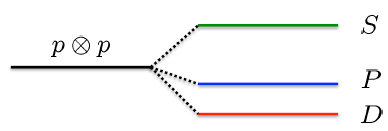
\includegraphics[scale=0.5]{ch1/image1}
\captionof{figure}{}
\end{center}
Nous avons précédemment discuté que
\begin{equation}
\mathcal{D}^{(0)} = S,\qquad\qquad\qquad\mathcal{D}^{(1)} = P
\end{equation}
Or
\begin{equation}
{\cal D}^{(l_1)} \otimes {\cal D}^{(l_2)} =
{\cal D}^{(l_1+l_2)} \oplus  {\cal D}^{(l_1+l_2-1 )} \oplus
\ldots \oplus {\cal D}^{(\vert l_1-l_2 \vert)}
\end{equation}
Dès lors
\begin{equation}
{\cal D}^{(1)} \otimes {\cal D}^{(1)} =
{\cal D}^{(2)} \oplus  {\cal D}^{(1)} \oplus
 {\cal D}^{(0)}
\end{equation}
Ou encore
\begin{equation}
p \otimes p =
D \oplus  P \oplus S
\end{equation}
Nous avons trois couple $j_1m_1$ pour le premier électron et trois pour le
second ($p_{0,\pm1}$). Au total, nous avons neuf couples possible. Nous avons
donc une matrice de représentation de dimension 9 car la base contient 9 fonction.
Nous avons réduit la représentation 9*9 (pour chaque triade $\omega$) que nous réduisons
en une somme de représentation irréductible : nous en avons trois ici.\\

Lorsque l'on fait $p\otimes p$, si l'on veut que l'hamiltonien soit invariant à la
rotation, le niveau $D$ sera dégénéré 5 fois, $P$ trois fois et $S$ une fois et non pas
un niveau 9 fois.}\ \\

	\begin{wrapfigure}[8]{r}{3cm}
	\vspace{-5mm}
	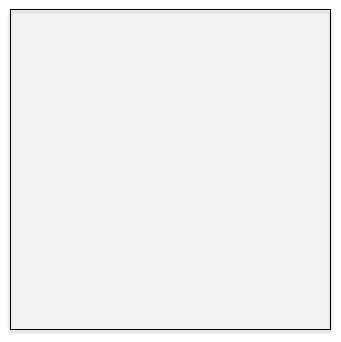
\includegraphics[scale=0.4]{ch1/image2}
	\captionof{figure}{ }
	\end{wrapfigure}
Expliquons d'une façon plus visuelle. Nous avons, dans la représentation découplée
\begin{equation}
\vert j_1 m_1 j_2 m_2  \rangle \equiv 
\vert j_1 m_1 \rangle \vert j_2 m_2 \rangle 
= \vert j_2 m_2 \rangle  \vert j_1 m_1 \rangle
\end{equation}
\begin{equation}
\vert p m_1 p  m_2  \rangle \equiv 
\vert p m_1 \rangle \vert p m_2 \rangle
\end{equation}

Et ceci pour n'importe quelle triade $\omega$. De plus
\begin{equation}
\vert p m_1 p  m_2  \rangle \} =
\{
\vert p_{+1} p_{+1} \rangle ,
\vert p_{+1} p_{0} \rangle , 
\ldots
\vert p_{-1} p_{-1} \rangle \}
\end{equation}
\begin{equation}
g = (2j_1 + 1)(2j_2 +1) = 3^2 = 9
\end{equation}
\ \\

	\begin{wrapfigure}[4]{r}{3cm}
	\vspace{-5mm}
	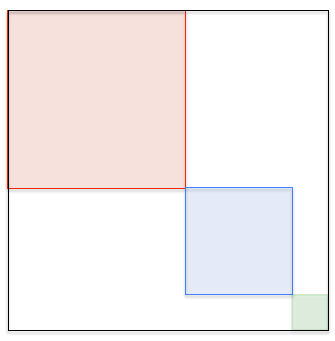
\includegraphics[scale=0.4]{ch1/image3}
	\captionof{figure}{ }
	\end{wrapfigure}
Nous pouvons changer de représentation et passer à la représentation couplée en 
définissant $\vec{j} = \vec l_1+\vec l_2$
\begin{equation}
\vert j_1 j_2 j m \rangle = 
\sum_{m_1,m_2} \vert j_1 m_1 j_2 m_2 \rangle 
{\color{red} 
\langle  j_1 m_1 j_2 m_2  \vert j_1 j_2 j m \rangle 
}
\end{equation}
Nous avons une matrice de dimension 5, une de 3 et une de 1. 
\begin{equation}
g = \sum_{j=\vert j_1 - j_2 \vert}^{ j_1 + j_2}
(2j+1)=
{\color{red}  5}  
+ {\color{blue}  3}  
+ {\color{green}  1} = 9
\end{equation}
Il y a des zéros, car ces matrices
sont irréductibles, on ne peut pas trouver une transformation qui fait mieux que cette 
diagonalisation. Le prix à payer c'est qu'il faut construire ces états
\begin{equation}
\{
{\color{red} 
\vert ppD_{+2} \rangle ,
\vert ppD_{+1}  \rangle , 
\ldots
\vert ppD_{-2}  \rangle } \},\quad
\{
{\color{blue} 
\vert ppP_{+1} \rangle ,
\vert ppP_{0}  \rangle , 
\vert ppP_{-1}  \rangle }  \},\quad
\{
{\color{green} 
\vert ppS_{0}  \rangle }
 \}
\end{equation}
Les différents blocs sont irréductibles : ils peuvent avoirs des éléments nuls mais ils sont
découplées des autres blocs, ça on est certain. Pour l'infinité d'opérateurs de rotation, on
ne peut pas faire mieux.

\exemple{\textsc{exercice slide 10-11}. Voir notes, sur le calcul des CG.}


\section{Coupling history of two angular momenta}
\textit{C'est l'histoire de deux moments angulaires}. Nous allons voir que l'histoire du 
couplage à de l'importance. Nous avons
\begin{equation}
\vert{\color{red} j_1 j_2} j m \rangle = 
\sum_{m_1,m_2} \vert j_1 m_1 j_2 m_2 \rangle \langle 
j_1 m_1 j_2 m_2 
\vert j_1 j_2 j m \rangle
\end{equation}
Nous avons aussi ceci, qui n'est \textbf{pas} la même chose : lorsque l'on couple deux moments
angulaires, l'ordre du couplage est capital
\begin{equation}
\begin{array}{ll}
\vert {\color{red} j_2  j_1} j m \rangle &= \DS
\sum_{m_2, m_1} \vert j_2 m_2 j_1 m_1 \rangle \langle 
j_2 m_2 j_1 m_1
\vert j_2 j_1 j m \rangle\vspace{2mm}\\
&=\DS 
\sum_{m_2, m_1} \vert j_1 m_1 j_2 m_2 \rangle \langle 
j_2 m_2 j_1 m_1
\vert j_2 j_1 j m \rangle
\end{array}
\end{equation}
Dans le \textit{ket} de la somme on peut intervertir $j_1$ et $j_2$ pour retrouver
le même \textit{ket} que dans la première histoire. Cependant, les coefficients de 
CG sont différents
\begin{equation}
\langle j_1 m_1 j_2 m_2 \vert j_1 j_2 j m \rangle 
= (-1)^{j_1 - j_2 + m} \sqrt{2j+1} \left(
\begin{array}{ccc}
j_1 & j_2 & j \\
m_1 & m_2 & -m 
\end{array} \right)
\end{equation}
\begin{equation}
\langle j_2 m_2 j_1 m_1 \vert j_2 j_1 j m \rangle 
= (-1)^{j_2 - j_1 + m} \sqrt{2j+1} \left(
\begin{array}{ccc}
j_2 & j_1 & j \\
m_2 & m_1 & -m 
\end{array} \right)
\end{equation}
On peut exprimer l'un en fonction de l'autre, moyennant l'introduction d'un facteur de phase
\begin{equation}
\left( \begin{array}{ccc} j_2 & j_1 & j \\ m_2 & m_1 & -m 
        \end{array} \right)
= (-1)^{j_2 + j_1 +j}
\left( \begin{array}{ccc}
j_1 & j_2 & j \\
m_1 & m_2 & -m 
\end{array} \right)
\end{equation}

Résumons. Tout $j$ a une "histoire". 
\begin{equation}
\left\{ \begin{array}{l}
{\bf j}^2 \; \vert  {\color{red}  \alpha} j m \rangle  
=  \hbar^2 j(j + 1) \vert  {\color{red}  \alpha}  j m \rangle \\
j_{z} \; \vert  {\color{red}  \alpha}  j m \rangle  
=  \hbar m  \; \vert {\color{red}  \alpha}   j m \rangle  
 \end{array} \right.
\end{equation}
Ici elle est triviale, c'est celle de deux moments angulaires. Il y a deux scénarios possibles : $\alpha$ ou $\beta$ qui diffèrent d'un \textbf{facteur de phase}
\begin{equation}
\vert \overbrace{j_1 j_2}^{\alpha} j m \rangle = 
{\color{red} 
(-1)^{j_1 + j_2 -j}    }
\vert \overbrace{j_2 j_1}^{\beta}j m \rangle
\end{equation}
C'est presque la même chose, mais il y a une phase. $L+S$ n'est pas la même chose que $S+L$, c'est
qu'une phase mais elle est très importante
\begin{equation}
\vert L S J M \rangle = 
{\color{red}  (-1)^{L + S - J}  }
 \vert S L J M \rangle
\end{equation}


\subsection{Application : deux électrons - tous les états ne sont pas autorisés}
Prenons deux spins : $j_1$ le spin du premier et $j_2$ le spin du second. Il y a indiscernabilité
des particules : si on met l'électron 1 dans un tel état et l'autre dans le même, je peux me
permettre de faire l'inverse et je ne pourrai pas faire la différence. Pour discuter, il faut tout
de même les labelliser. Construisons une fonction symétrique par rapport à l'échange
\begin{equation}
\chi^+_{SM_S} = \frac{1}{\sqrt{2}} [ \chi_{SM_S} (1,2) + \chi_{SM_S} (2,1) ]
\end{equation}
Avec ces deux spins, on va créer un état de spin total $S$ avec une projection $M_S$. Avec 
deux spins on peut faire l'état singlet ou triplet. On va écrire la second terme en fonction du premier, mais ce n'est pas la même fonction : il y a un facteur de phase. \\

La mise en évidence va faire apparaître l'interférence entre les deux
\begin{equation}
\chi^+_{SM_S} = \frac{1}{\sqrt{2}} [ \chi_{SM_S} (1,2) + (-1)^{1-S}  \chi_{SM_S} (1,2) ]
\end{equation}
L'état peut ainsi s'annuler
\begin{equation}
 \left\{ \begin{array}{ll}
\neq 0   &  \mbox{si}~S=1~\mbox{(triplet)} \\
= 0   &  \mbox{si}~S=0~\mbox{(singulet)} 
\end{array} \right.
\end{equation}
Si $S=1$, l'état de spin est totalement \textbf{symétrique} : c'est le \textbf{triplet}. Rien
qu'en regardant le spin, on a pu se convaincre qu'en construisant une propriété symétrique par
rapport à l'échange, cette fonction ne peut être que triplet par effet d'interférence entre les
deux composantes. \\

On peut faire la même chose pour une fonction antisymétrique par rapport à l'échange. L'état de 
spin qui est \textbf{antisymétrique} par rapport à l'échange est le \textbf{triplet}.\\

La fonction
d'onde devant être antisymétrique, la partie spatiale aura la symétrie adaptée. Pour un
\textbf{singlet} ($S=0$)
\begin{equation}
\Psi_{LM_L 00}(q_1,q_2) = \chi^{-}_{00}(1,2) \times  \frac{1}{\sqrt{2}} [ \psi_{ll' LM_L} ({\bf r}_1, {\bf r}_2)+
(-1)^{l+l'-L}  \psi_{l'lLM_L} ({\bf r}_1, {\bf r}_2) ]
\end{equation}
Pour un \textbf{triplet} ($S=1$)
\begin{equation}
\Psi_{LM_L 1M_S}(q_1,q_2) = \chi^{+}_{1M_S}(1,2) \times  \frac{1}{\sqrt{2}} [ \psi_{ll' LM_L} ({\bf r}_1, {\bf r}_2) -
(-1)^{l+l'-L}  \psi_{l'lLM_L} ({\bf r}_1, {\bf r}_2) ]
\end{equation}

\subsubsection{Différence entre $2p3p$ et $2p^2$}
Réécrivons ce que nous venons de dire, en combinant les parties spatiales et de spins pour avoir
une fonction antisymétrique à l'échange. 
\begin{equation}
\Psi_{nl n'l' LM_LSM_S}(q_1,q_2) =\frac{1}{\sqrt{2}} 
\left\{ 
R_{nl}(r_1) R_{n'l'}(r_2)
 \Psi_{l_1 l'_2  LSM_LM_S} 
+ (-1)^{l+l'-L-S} 
R_{nl}(r_2) R_{n'l'}(r_1)
 \Psi_{l'_1 l_2 LSM_LM_S}  \right\}
\end{equation}
Deux cas sont possible
\begin{enumerate}
\item SI $nl\neq n'l'$, on ne peut rien mettre en évidence car les parties radiales sont différentes,
on ne pourra pas faire ressortir un facteur commun. 
\begin{equation}
2p3p\Rightarrow \; ^3D, \; ^1D, \; ^3P, \; ^1P, \; ^3S, \; ^1S
\end{equation}
\item Si $nl=n'l'$ (deux électrons dans la même couche), on va pouvoir procéder à une mise en 
évidence
\begin{equation}
\Psi_{nl^2 LM_LSM_S}(q_1,q_2) = R_{nl}(r_1) R_{nl}(r_2)
 \Psi_{l_1 l_2 LSM_LM_S} 
\frac{1}{2} 
\left\{ 1 
+ (-1)^{2l-L-S}\right\}
\end{equation}
Nous allons avoir un phénomène d'interférences : certains états vont s'annuler. Cette fonction 
est antisymétrique à l'échange et va s'\textbf{annuler} si $(L+S)$ est impair, tout bêtement à 
cause de ce facteur de phase.
\begin{equation}
2p^2 \Rightarrow\ ^1D,\ ^3P,\ ^1S
\end{equation}
\end{enumerate}

Lorsque nous avons fait le couplage $2p3p$, les électrons diffèrent déjà de nombres quantiques. Tout
est permis et on peut utiliser les règles d'addition vectorielles. La répulsion de coulomb entre les 
électrons nous force à couplée $l_1,l_2,s_1$ et $s_2$ mais en plus la fonction doit être 
antisymétrique par rapport à l'échange (fermion).\\

Si les électrons sont équivalent, l'interférence va se manifester et certains états (comme le 
triplet $S$) ont disparus. C'est normal car le sudoku n'est plus \textit{un électron dans six 
boîtes et un autre dans six boîtes}(ce qui donne 36) mais \textit{deux particules dans six
boîtes} (ce qui donne 15). Le fait que l'on ai forcé l'antisymétrie par rapport à l'échange à 
forcé certains termes à s'annuler.

\section{Coupling of three angular momenta}
Pour coupler trois moments angulaires, il va falloir décomposer\footnote{Notes \textit{slide 19}}. On
réalise rapidement qu'il y a beaucoup d'histoires possible. On pourrait coupler $j_1$ à $j_2$ pour
former $J'$ et qu'lon couple à $j_3$ (histoire $\alpha$) ou encore coupler $j_2$ et $j_3$ 
pour former $J''$ que l'on couple à $j_1$. L'état final n'est forcément pas le même, car il a une histoire (l'ordre de couplage). 
\begin{center}
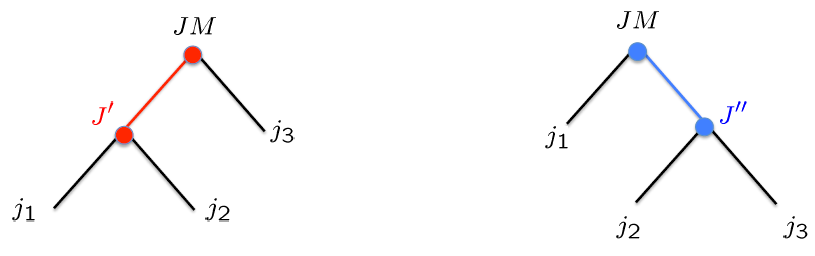
\includegraphics[scale=0.45]{ch1/image4}
\captionof{figure}{}
\end{center}
On s'intéresse à l'histoire $\alpha$
\begin{equation}
  \vert 
\overbrace{ [(j_1 j_2) {\color{red} J'}, j_3 ]}
^{ {\color{red} \alpha}} 
J M \rangle
\end{equation}
A chaque vertex (boule), les inégalités triangulaires doivent être vérifiées. On va essayer de
relier cette première histoire à l'histoire $\beta$
\begin{equation}
  \vert \overbrace{[ j_1, (j_2 j_3) {\color{blue} J''}] }
^{{\color{blue} \beta}}
J M \rangle
\end{equation}
Comment les relier? Avec le relation de fermeture, nous pouvons toujours écrire que
\begin{equation}
\ket{[(j_1j_2)J',j_3]JM} = \sum_\beta \ket\beta\bra\beta\ket{[(j_1j_2)J',j_3]JM}
\end{equation}
Nous voulons $\beta$, c'est l'histoire que l'on recherche.  Dans la précédente expression,
$J,M$ sont les mêmes, tout comme $j_1$ et $j_2$ qui sont fixés. On n'a pas d'autre choix que
de sommer sur $J''$
\begin{equation}
\vert 
 [\underline{(j_1 j_2) {\color{red} J'}}, j_3 ]J M \rangle= \sum_{ {\color{blue} J''}} 
\vert [ j_1, (j_2 j_3) {\color{blue} J''}]  
J M  \rangle
 \langle  [ j_1, (j_2 j_3) {\color{blue} J''}]  
J M \vert 
[(j_1 j_2) {\color{red} J'}, j_3 ]J M \rangle
\end{equation}
Comment pouvons-nous calculer le terme souligné ? Avec un CG !
\begin{equation}
\ket{(j_1j_2)J'M'} = \sum_{m_1m_2} \ket{j_1m_1j_2m_2}\bra{j_1m_1j_2m_2}\ket{(j_1j_2)J'M'}
\end{equation}
Ainsi, pour coupler le 3ème, on va re-sommer
\begin{equation}
\ket{[(j_1j_2),j_3]JM} = \sum_{M'm_3}\ket{(j_1j_2)J'M'j_3m_3}\bra{(j_1j_2)J'M'j_3m_3}
\ket{[(j_1j_2),j_3]JM}
\end{equation}
On peut faire la même chose et exprimer l'histoire $\beta$ en fonction de $\alpha$
\begin{equation}
\begin{array}{ll}
  \vert [ j_1, (j_2 j_3) {\color{blue} J''}]  J M \rangle 
&=\DS
\sum_{\alpha} \vert \alpha JM \rangle \langle \alpha JM
\vert [ j_1, (j_2 j_3) {\color{blue} J''}]  J M \rangle\vspace{2mm}\\
&\DS=
\sum_{{\color{red} J'}} \vert [ (j_1 j_2) {\color{red} J'}, j_3 ]
JM \rangle \langle [ (j_1 j_2) {\color{red} J'}, j_3 ] JM
\vert [ j_1, (j_2 j_3) {\color{blue} J''}]  J M \rangle
\end{array}
\end{equation}

Le coefficient de recouplage est donné par
\begin{equation}
\langle [ (j_1 j_2) {\color{red} J'}, j_3 ] JM
\vert [ j_1, (j_2 j_3) {\color{blue} J''}]  J M \rangle =
(-1)^{j_1 + j_2 + j_3 + J} [J',J'']^{1/2}
\left\{
\begin{array}{ccc}
{\color{red} J'}  &  j_3   &   J \\
{\color{blue} J''} &  j_1  & j_2  \end{array}  \right\}
\end{equation}
Lorsque l'on regarde à droite, $M$ n'intervient pas. La transformation unitaire est 
la même pour toute valeur de $M$ (démontré en annexe). Le coefficient de couplage ne dépend 
que d'un $6j$ : le total, les trois que l'on couple et les deux intermédiaires. Ce terme est un scalaire et \textsc{Wigner} 
s'est intéressé à avoir une notation compacte. Il a alors introduit le $6j$, car six moments
angulaires.\\

Le $6j$ contient les quatre règles triangulaires qui viennent des quatre vertex
\begin{equation}
\left\{ \begin{array}{ccc}
\bullet  & \bullet & \bullet \\ \cdot & \cdot & \cdot \end{array} 
\right\},
\left\{ \begin{array}{ccc}
\bullet  & \cdot & \cdot \\ \cdot & \bullet & \bullet \end{array} 
\right\},
\left\{ \begin{array}{ccc}
\cdot & \bullet & \cdot \\ \bullet & \cdot & \bullet \end{array} 
\right\},
\left\{ \begin{array}{ccc}
\cdot & \cdot & \bullet \\ \bullet & \bullet & \cdot \end{array} 
\right\}
\end{equation}
Ils possèdent un tas de propriétés intéressantes, reprises au \textit{slide 22}.\\

Ré-insistons sur l'expression suivante
\begin{equation}
\langle [ (j_1 j_2) {\color{red} J'}, j_3 ] JM
\vert [ j_1, (j_2 j_3) {\color{blue} J''}]  J M \rangle=
(-1)^{j_1 + j_2 + j_3 + J} [J',J'']^{1/2}
\left\{
\begin{array}{ccc}
{\color{red} J'}  &  j_3   &   J \\
{\color{blue} J''} &  j_1  & j_2  \end{array}  \right\}
\end{equation}
où $[J',J''] = \sqrt{(2J'+1)(2J''+1)}$. Ces coefficients de recouplage sont bien
\textbf{indépendants de $M$} : c'est très intéressant car ce coefficient sera le même
pour chaque valeur de $M$
\begin{equation}
\langle [ (j_1 j_2) {\color{red} J'}, j_3 ] JM
\vert [ j_1, (j_2 j_3) {\color{blue} J''}]  J M \rangle
= 
\langle [ (j_1 j_2) {\color{red} J'}, j_3 ] J
\vert [ j_1, (j_2 j_3) {\color{blue} J''}]  J  \rangle 
\end{equation}
$$-J \le M \le +J$$


\subsubsection{Example: levels of np(n+1)s in atoms of Groupe IVA}
En guise d'application, regardons comment on pourrait définir une transformation unitaire
qui permettra de discuter la distribution des niveaux entre deux systèmes différents. Nous
prenons les tables du \textsc{nist} et on regarde pour le carbone et le plomb. \\

	\begin{wrapfigure}[12]{l}{9cm}
	\vspace{-5mm}
	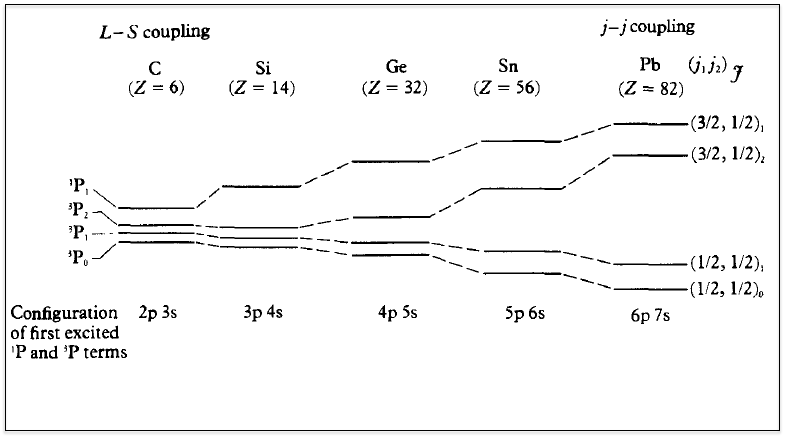
\includegraphics[scale=0.4]{ch1/image5}
	\captionof{figure}{ }
	\end{wrapfigure}
Pour le carbone, on part de zéro (tout en haut du tableau, \textit{slide 24}) jusqu'à 
l'ionisation. Tout un coup, un terme $2p3s$ arrive avec des niveaux très rapprochés. On a du
carbone $1s^22s^22p3s$. Si on fait d'abord interagir, on trouve $\vec{L}=\vec1+\vec0$ donnant
un état $^1P$ et un état $^3P$. Ensuite, on fait intervenir le spin-orbite en effectuant
$\vec{L}+\vec S=\vec J$ qui va faire apparaitre les niveaux entourés en rouge. Ici, on peut voir
le S-O comme une perturbation\footnote{Notes \textit{slide 24}.}\\

Pour le plomb, la situation que l'on observe expérimentalement est différente. Ici, c'est le 
S-O qui a d'abord été appliqué ($\vec{j_i}=s_i+l_i$) puis l'interaction entre les deux
($j=j_1+j_2$) : l'interaction est vue comme une perturbation\footnote{Voir note \textit{slide 28}}.\\

La figure ci-dessus, à gauche, montre ce qui se passe entre le carbone et le plomb, on a une
"lecture des niveaux". A gauche, il semble que le couplage $L-S$ est la perturbation alors qu'à
droite, c'est plus l'interaction qui peut être vue comme une perturbation\footnote{Voir notes
\textit{slide 24}, cours 3. Voir aussi les notes sur le pdf, \textit{slide 29}.}

\subsection{Balance between  Coulomb repulsion and spin-orbit interaction}
Nous avons l'hamiltonien suivant
\begin{equation}
H = \sum_{i=1}^N h(i)  
{ \color{blue}+ \sum_{i < j}^N \frac{1}{r_{ij}}}
{\color{red}+  \sum_{i=1}^N \xi_i(r_i) {\bf l}_i 
\cdot  {\bf s}_i }
\end{equation}
où $h(i)  = - \frac{1}{2} \nabla_i^2 -  \frac{Z}{r_i}$. Il y a deux façon de le partitionner. On 
peut voir l'interaction coulombienne comme une perturbation et partir du spin-orbite (cas 2) ou faire 
l'inverse : partir de l'interaction coulombienne et considérer que le perturbation est le spin
orbite (cas 1). Les deux cas sont les suivants :
\begin{itemize}
\item[$\bullet$] $H = H^0 {\color{blue} + V}$
\begin{equation}
H^0 = \sum_{i=1}^N h(i)  
+ \sum_{i < j}^N \frac{1}{r_{ij}},\qquad\qquad
V =  \sum_{i=1}^N \xi_i(r_i) {\bf l}_i \cdot  {\bf s}_i 
\end{equation}
\begin{equation}
\Psi^{(0)} = 
  \vert \overbrace{[ l_2, (s_1 s_2) {\color{blue} S}] }
^{{\color{blue} \beta}}
J M \rangle
\end{equation}
\item[$\bullet$] $H = \tilde{H}^0 {\color{red} + \tilde{V}}$
\begin{equation}
\tilde{H}^0 = \sum_{i=1}^N h(i)  
+  \sum_{i=1}^N \xi_i(r_i) {\bf l}_i \cdot  {\bf s}_i,\qquad\qquad
{\color{red}
\tilde{V} =  \sum_{i < j}^N \frac{1}{r_{ij}}  }
\end{equation}
\begin{equation}
\tilde{\Psi}^{(0)} = 
  \vert 
\overbrace{ [ s_1, (l_2 s_2) {\color{red} j_2} ]}
^{{\color{red} \alpha}} 
J M \rangle
\end{equation}
\end{itemize}
Dans le plomb, les électrons tournent plus vite et sont ainsi plus relativiste : l'interaction
la plus importante est le spin-orbite, nous sommes dans le second cas. Par contre, pour le carbone,
le spin-orbite est petit et coulomb domine (cas 1). \\

Lorsque l'on fait une observation, on a accès au "vrai" hamiltonien, que l'on essaye d'approcher. 
Lorsque l'on utilise $\beta$, on diagonalise $H_0$ sans l'interaction S-O. Ce choix de base peut
être excellent, il va représenter le spectre de $H_0$ dans cette base la. Si on ne mets pas de
S-O, on obtient le singlet $P$ et le triplet $P$. Ceci suppose que $\beta$ est parfait. S'il n'y a
pas de S-O dans $\beta$, on n'est pas forcée de construire $J$ : le rajout du S-O ne modifiera que
peu les niveaux.\\

Que l'on choisisse l'histoire $\alpha$ ou $\beta$, les valeurs propres sont les mêmes car la base
est complète. Pourquoi on se tracasse alors ? Quel est l'intérêt du choix de la base? Pour calculer
les valeurs propres, il n'y aura pas de problème. On avait des légères pollutions : dans une base
les proportions de pollutions seront plus faible, mais dans l'autre elles seront énormes (par 
exemple, si on prend Coulomb comme perturbation dans le plomb, elle sera énorme). Ce n'est donc
pas un problème pour l'énergie, mais pour les vecteurs propres. Si on diagonalise dans la mauvaise
base, on ne pourra pas dire si on est triplet ou singlet $P$.\\

Quelle est donc la "bonne" base ? On parle de nombre quantique parfait quand les vecteurs propres
de $H$ (après diagonalisation) sont les fonctions propres de la base. Si ce n'est pas parfait, on 
aura un mélange des éléments de la base. Ici, c'est $J^2$ qui commute avec les deux histoires : 
c'est un bon nombre quantique car, quelque soit l'histoire, c'est le \textbf{même} 
$J$\footnote{Pour le \textit{slide 29}, voir notes pdf et manuscrites, pas mal de choses "extra".}.\\

	\begin{wrapfigure}[8]{l}{9cm}
	\vspace{-5mm}
	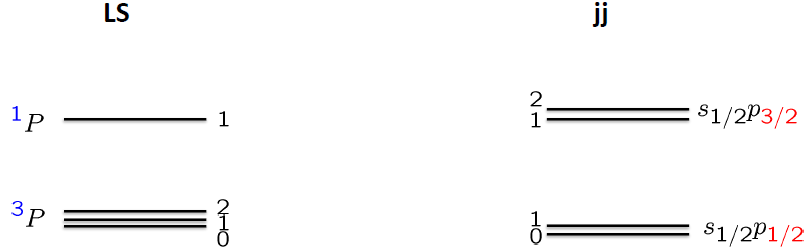
\includegraphics[scale=0.4]{ch1/image6}
	\captionof{figure}{ }
	\end{wrapfigure}
Comment peut-on corréler l'histoire de gauche à celle de droite ? Quel est le nombre quantique 
qui est parfait ? $J$, ou éventuellement $M$ qui est derrière. Mais $M$ en l'absence de $B$ 
ne lève pas la dégénérescence, on n'en tient pas compte. Nous allons jouer à \textit{Dieu}. On va
faire $c\to\infty$ afin de ne plus avoir d'interaction spin-orbite (qui est un effet relativiste).
S'il n'y a pas de spin-orbite, "à gauche" on peut écraser les trois niveaux et on n'en aura plus 
que deux. On écrase aussi à droite\footnote{La, je l'ai pas. On n'aurait plus que un niveau alors?}.
Pourquoi $J$ est bien? Car il commute avec $H$ qui contient tout
\begin{equation}
\hat H\ket{\alpha JM} = E_{JM}\ket{\alpha JM}
\end{equation}
où l'énergie est indépendante de $M$ : $E_J$. Chaque fois que l'on a une valeur de $J$, elle est
certaine : quel que soit la configuration que \textit{Dieu} choisi avec ses potentiomètre, elle commutera. On peut imaginer avoir un degré de liberté qui varie de façon continue : on règle
comme on veut l'interaction coulombienne. La seule chose qui doit rester vrai, c'est que si
on a $J=2$ à gauche, on doit avoir la même chose à droite. On peut corréler les différentes
valeurs de $J$, mais une chose est impossible. On peut montrer qu'en mécanique quantique, 
\textbf{deux états de même symétrie ne se croisent jamais}.
\begin{center}
	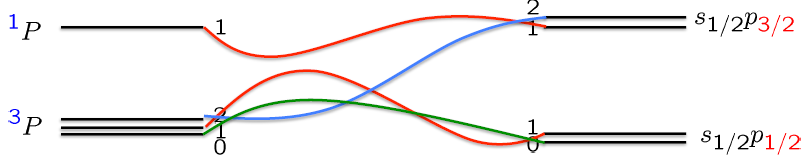
\includegraphics[scale=0.4]{ch1/image7}
	\captionof{figure}{ }
\end{center}
Essayons de comprendre. Nous avons quatre valeurs de $J$ à corréler (2,0,1,1). Regardons pour
chacun des cas
\begin{enumerate}
\item $J=2$. On n'a qu'un seul état $J=2, M=2$, on ne forme qu'un bloc (les états de différents $J$ 
n'interagissent pas. Il n'y a donc qu'un bloc et $H$ donnera l'énergie multiplié par une fonction. 
Comme il n'y a qu'un seul bloc, on ne peut avoir que le $sp\ ^3P_2$.\footnote{On effet, on doit 
avec $J=L+S$ et comme $L=1$, il faut que $S=1$ (triplet).} A droite, il n'y a qu'un
seul $J=2$, mais la base c'est $s_{1/2}p_{3/2}$.
\begin{equation}
  \vert sp \; ^{{\color{blue} 3}}P_2 \rangle  
=
\vert s_{1/2} p_{{\color{red} 3/2}} \; J=2  \rangle
\end{equation}
\item $J=0$. On peut prendre la base de gauche ou de droite, c'est rigoureusement le même 
\textit{ket}. Il n' y a pas de mélange possible. Que ce soit $C$ ou $Pb$, on n'a que lui
\begin{equation}
  \vert sp \; ^{{\color{blue} 3}}P_0 \rangle  
=
\vert s_{1/2} p_{{\color{red} 1/2}} \; J=0  \rangle
\end{equation}
\item $J=1$. Ici, il n'y a plus que un choit. A gauche, on aura un mélange de $^3P$ et 
$^1P$ (ou $a \gg b$ pour cet état-là, le spin-orbite du carbone étant très petit\footnote{Pourquoi?}.
\begin{equation}
\Psi_1 = a 
  \vert sp \; ^{{\color{blue} 3}}P_1 \rangle
+ b
  \vert sp \; ^{{\color{blue} 1}}P_1 \rangle
=
\alpha
  \vert s_{1/2} p_{{\color{red} 1/2}} \; J=1  \rangle
+ \beta
  \vert s_{1/2} p_{{\color{red} 3/2}} \; J=1  \rangle
\end{equation}
A droite, ce sera sûrement un mélange des deux $J=1$ mais avec $\alpha\gg \beta$. Le nom du 
vecteur est important, si on en nomme un $s_{1/2}p_{1/2}$ et pas $^3P$ c'est que ça a de 
l'importance : $J=1$ n'est pas suffisant.
\item $J=1$. Il s'agit aussi d'un mélange
\begin{equation}
\Psi_2 = b 
  \vert sp \; ^{{\color{blue} 3}}P_1 \rangle
-a
  \vert sp \; ^{{\color{blue} 1}}P_1 \rangle
=
\beta
  \vert s_{1/2} p_{{\color{red} 1/2}} \; J=1  \rangle
- \alpha
  \vert s_{1/2} p_{{\color{red} 3/2}} \; J=1  \rangle
\end{equation}
Pourquoi utiliser $(\alpha,\beta)$?
\end{enumerate}
Comment pouvons nous trouver $(a,b)$ ou $(\alpha,\beta)$? Il faut chercher la transformation
unitaire qui diagonalise. Pour cela, on va chercher les valeurs propres en annulant le 
déterminant séculaire. Le détail est donné aux \textit{slide 42-43}\footnote{Lire notes 
cours 3, \textit{slide 42}}.

\begin{equation}
E_{1,2} 
= E_\pm =\frac{H_{11} + H_{22}}{2}
% \pm \sqrt{
%\left( \frac{H_{22} - H_{11}}{2} \right)^2 + H_{12}H_{21}
\; \pm \;  H_{12} \sqrt{
\left( \frac{H_{22} - H_{11}}{2 H_{12}} \right)^2 + 1
}
\end{equation}

Étudions les deux cas limites. Nous avons au départ 
\begin{equation}
\left(\begin{array}{cc}
H_{11}&H_{12}\\
H_{21}&H_{22}
\end{array}\right)
\end{equation}
Lorsque l'on va diagonaliser, $H_{22}$ nous donnera l'énergie $E_2$ et $H_{11}$ 
l'énergie $E_1$ (l'un va monter et l'autre descendre, voir notes \textit{slide 44}). Les termes
non-diagonaux traduisent l'interaction. Il y a donc deux cas limites
\begin{enumerate}
\item ${\color{red} \Delta \equiv 
\frac{H_{12}}{H_{11}-H_{22}} \ll 1 }$. Une des énergies va un peu monter, et l'autre un peu
descendre. On trouve respectivement
\begin{equation}
E^+ \approx H_{11} + \dfrac{H_{12}^2}{H_{11}-H_{22}},\qquad\qquad
\left(\begin{array}{c}
1-\Delta^2/2\\
\Delta
\end{array}\right)
\end{equation}
\begin{equation}
E^- \approx H_{22} - \dfrac{H_{12}^2}{H_{11}-H_{22}},\qquad\qquad
\left(\begin{array}{c}
\Delta\\
-1+\Delta^2/2
\end{array}\right)
\end{equation}
L'un vaut presque 1 et l'autre presque -1, mais ils sont un peu contaminés l'un par l'autre. Ces
deux états se sont poussés (l'un est un peu monté, l'autre un peu descendu) mais on peut toujours
associer $H_{11}$ à $E_1$, \dots 
\item ${\color{red} 
\vert \Delta \vert \equiv 
\left\vert 
\frac{H_{12}}{H_{11}-H_{22}} \right\vert  \gg 1}$. Ce second scénario est nettement plus 
dramatique car si $H_{11}\approx H_{22}$, $\Delta$ peut devenir grand. Si on diagonalise une
matrice qui rempli cette condition ? On va voir apparaître la moyenne des deux et une énergie
va monter, l'autre descendre. Quel que soit $H_{12}$, c'est la catastrophe.
\begin{equation}
E^\pm
 \simeq
\frac{H_{11} + H_{22}}{2} \pm H_{12},\qquad\qquad\left( 
\begin{array}{c}
1/ \sqrt{2} \\ \pm  1/ \sqrt{2}  \end{array} \right)
\end{equation}
\end{enumerate}

\subsubsection{Résumons}
	\begin{wrapfigure}[16]{l}{9cm}
	\vspace{-5mm}
	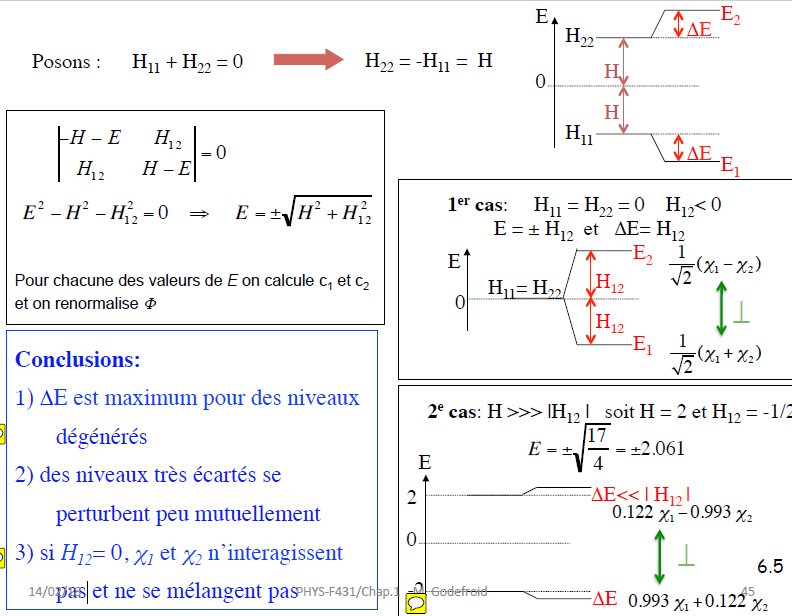
\includegraphics[scale=0.4]{ch1/image8}
	\captionof{figure}{ }
	\end{wrapfigure}
Posons
\begin{equation}
H_{11}+H_{22}=0\Rightarrow H_{22}=-H_{11}=H
\end{equation}
et considérons $\Delta E$, la variation par rapport au cas non-dégénéré.
Sur la droite, on retrouve les deux cas. Si $H_{11}=H_{22}=0$, les deux niveaux sont
dégénérés et $\Delta E$ sera maximal : la contamination est de 50/20. Par contre, si les
deux niveaux sont initialement très écartés, la perturbation sera faible. Il y a toujours
un peu de contamination mais le vecteur propre est presque pur (loin du 50/50 du cas dégénéré).
De même, s'il n'y a pas de terme non-diagonal dans $H$, il n'y aura pas d'interaction ni de 
mélange. En effet, il n'y a pas d'interaction entre $J=1$ et $J=2$ : ils sont seuls car les
blocs n'interagissent pas.

\newpage
Maintenant que l'on sait ça, reprenons. Pour $J=0$, les deux bases étaient parfaites car la
perturbation $V$ ou $\tilde{V}$ est diagonale, il n'y a donc pas de couplage. Ces états sont
purs dans les deux bases et donc forcément égaux. Pour $J=2$, même conclusion.\\

Par contre, pour $J=1$, la base peut être bonne, mauvaise, mais jamais parfaite. Ici, 
$V$ ou $\tilde{V}$ couple les fonctions de base (mais le croisements des états de même
symétrie est évité par la diagonalisation).

\subsubsection{Groupe IVA $np(n+1)s$}
En allant de la limite $LS$ vers la limite $jj$, l'état $J=1$ le plus bas $(^3P)$ est 
de plus en plus mélange à l'état singulet $^1P_1$. A la limite $jj$, cet état a acquis 
33\% de caractère singulet, mais reste $^3P$ à 66\%. Ce même état correspond à un état 
pur $(1/2,1/2)_1$. Le fait qu'il ne change pas de caractère dominant montre qu'il n'y
a pas eu de croisement évité.\\

	\begin{wrapfigure}[16]{l}{6cm}
	\vspace{-5mm}
	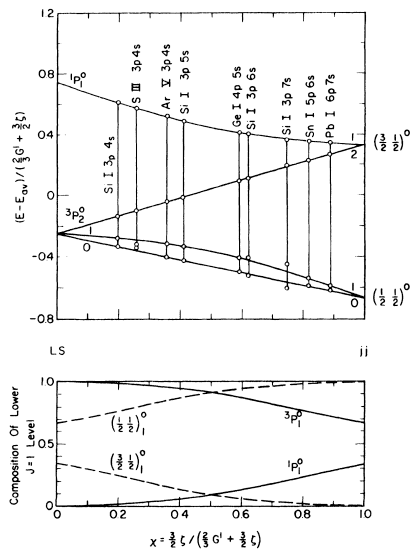
\includegraphics[scale=0.5]{ch1/image9}
	\captionof{figure}{ }
	\end{wrapfigure}
Sur le graphique du dessus, nous voyons que le triplet $P$ est totalement pur à gauche,
mais pas à droite. Pour le quantifier, regardons la composition du niveau $J=1$ le plus
bas. En haut à gauche se trouve l'état $^3P$ totalement pur. Si l'on suit la ligne pleine,
il reste triplet $P$ à 66\% à droite. On peut changer de base et prendre celle en 
pointillé. La, c'est à droite que le triplet $P$ sera 100\% pur : il vaut mieux ici utiliser
la base $\left(1/2,1/2\right)_1$ qui est pure (mais à ne pas utiliser à gauche. Dans l'abscisse du 
deuxième schéma, $G$ mesure la force de l'échange entre les deux électrons (intégrale
d'échange). Le spin-orbite, c'est $\zeta$. Si l'échange $\gg$ S-O, le dénominateur explose
et $\chi\to0$.\\

\exemple{Les \textit{slides 51-52} sont un exercice sur les matrices de recouplage. 
Voir notes cours 3.}

\subsubsection{Groupe VIIIA $np^5(n+1)s$}
	\begin{wrapfigure}[14]{r}{6cm}
	\vspace{-5mm}
	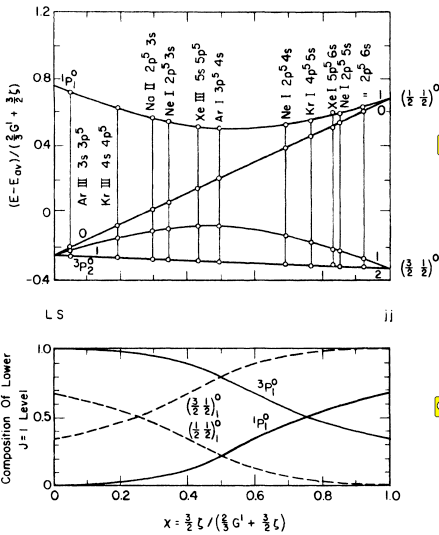
\includegraphics[scale=0.5]{ch1/image10}
	\captionof{figure}{ }
	\end{wrapfigure}
Comme pour $np(1+1)s$, en allant de la limite $LS$ vers la limite $jj$, l'état $J=1$ le
plus bas ($^3P$) est de plus en plus contaminé par le singulet $^1P_1$. A la limite 
$jj$, cet état a acquis \textbf{66\%} de caractère singulet est n'est plus $^3P$ que 
pour 33\%. Cet état correspond à un état pur $(3/2,1/2)_1$ (inversion de la structure
fine par rapport à $np(n+1)s$. Le fait qu'il \textbf{change de caractère dominant} est
la signature du croisement \textbf{évité}, comme le montre le mélange symétrique 50-50\%.\\

Dans le graphique du dessus, le singlet $P$ est au dessus à gauche et, en dessous à gauche,
on retrouve le singlet $P$ avec sa structure fine. A droite, on remarque que la structure
spin-orbite est grande pour le triplet $P$ qui "ne l'est donc plus". Si l'on regarde la 
composition (en dessous), quelque chose qui était dominant $^3P$ devient dominé $^1P$. 
Il y a un croisement dans la composition, ce qui montre que triplet et singlet ne sont pas des
bons nombres quantiques. Le 50-50\%, c'est le cas dégénéré. Or, pour $J=1$ si on regarde
le graphique du dessus, ce n'est pas dégénéré : on a évité le croisement.\\

Pour résumé
\begin{itemize}
\item[$\bullet$] Des états de \textbf{symétrie différentes} n'interagissent jamais et peuvent
donc se croiser.
\item[$\bullet$] Des états de \textbf{même symétrie} interagissent et ne peuvent pas se 
croiser après diagonalisation. Les deux états changent de label de part et d'autre du croisement
évité. Du point de vue de l'évolution de la composition des vecteurs prores, tout se passe
donc comme si les états se croisaient.
\end{itemize}


\section{Coupling of four angular momenta}
On s'intéresse maintenant au couplage de \textbf{quatre} moments angulaires
\begin{equation}
{\bf l}_1 +   {\bf  s}_1 + {\bf  l}_2 + {\bf  s}_2 = {\bf  J}
\end{equation}
On peut ici écrire quatre histoires différentes

\begin{multicols}{2}
\begin{description}
\item[LS]\ \\
$\begin{array}{ccc}
{\bf l}_1 +   {\bf  l}_2  & = & {\color{red} {\bf  L}} \\
{\bf s}_1 +   {\bf  s}_2  & = & {\color{red}{\bf  S}} \\
{\bf L} +   {\bf  S}  & = & {\bf  J}
\end{array}$
\item[LK]\ \\ $\begin{array}{ccc}
{\bf l}_1 +   {\bf  l}_2  & = & {\color{red}{\bf  L}} \\
{\bf L} +   {\bf  s}_1  & = & {\color{red}{\bf  K}} \\
{\bf K} +   {\bf  s}_2  & = & {\bf  J}
\end{array}$
\item[jK]\ \\ $\begin{array}{ccc}
{\bf l}_1 +   {\bf  s}_1  & = & {\color{red}{\bf  j}}_1 \\
{\bf j}_1 +   {\bf  l}_2  & = & {\color{red}{\bf  K}} \\
{\bf K} +   {\bf  s}_2  & = & {\bf  J}
\end{array}$
\item[jj]\ \\ $\begin{array}{ccc}
{\bf l}_1 +   {\bf  s}_1  & = & {\color{red}{\bf  j}}_1 \\
{\bf l}_2 +   {\bf  s}_2  & = & {\color{red}{\bf  j}}_2 \\
{\bf j}_1 +   {\bf  j}_2  & = & {\bf  J}
\end{array}$
\end{description}
\end{multicols}
On remarque que le nom de l'histoire correspond aux nombres quantiques
intermédiaires. Par exemple dans l'histoire $jj$, on couple le premier
S-O ($j_1$), puis le second ($j_2$) et enfin on tient compte de l'interaction
entre les deux ($J$). Évidemment, $J$ est le même dans toutes les histoires car
il s'agit d'un bon nombre quantique. On va pouvoir choisir la base.

\subsection{$pd$ dans un couplage $LS$}
	\begin{wrapfigure}[11]{r}{5cm}
	\vspace{-5mm}
	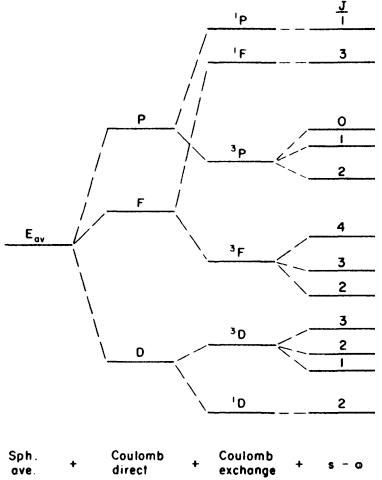
\includegraphics[scale=0.5]{ch1/image11}
	\captionof{figure}{ }
	\end{wrapfigure}
Nous avons ici un électron $p$, et un électron $d$ de valence. Si on pense
que $L$ et $S$ sont de bon nombres quantiques, on trouvera
\begin{equation}
P+D = \vec{1}+\vec 2 = 3,2,1\  (P, F, D)
\end{equation}
Il s'agit de l'effet coulombien direct : on ne peut pas différencier les 
triplets des singlets tant qu'on ne discute pas l'échange. Une fois l'échange
pris en compte, il faudra rajouter le spin-orbite (voir schéma ci-contre). Ceci
est conforme à l'histoire $LS$
\begin{equation}
\begin{array}{ccc}
{\bf l}_1 +   {\bf  l}_2  & = & {\color{red} {\bf  L}} \\
{\bf s}_1 +   {\bf  s}_2  & = & {\color{red}{\bf  S}} \\
{\bf L} +   {\bf  S}  & = & {\bf  J}
\end{array}
\end{equation}
Sur le spectre, nous avons bien créé tous les $J$ possibles. On peut vérifier
avec la dégénérescence
\begin{equation}
pd = \dfrac{6!}{1!(6-1)!}\dfrac{10!}{1!(10-1)!}=6*10=60
\end{equation}
Ceci correspond bien à 
\begin{equation}
\sum_{LS} g(LS) = \sum_{LS} (2L+1)(2S+1) = 60 = \sum_J g(J) = \sum_J(2J+1)
\end{equation}


\subsection{$pd$ dans un couplage $jj$}
Cette fois-ci, on va coupler les $j$. Par exemple $\vec l_2+s_2= \vec 2 + \vec{1/2} =\vec j_2 \to
j_2=3/2,5/2$. On couplera ensuite avec $j_1$, pour donner $j$
\begin{equation}
\begin{array}{ccc}
{\bf l}_1 +   {\bf  s}_1  & = & {\color{red}{\bf  j}}_1 \\
{\bf l}_2 +   {\bf  s}_2  & = & {\color{red}{\bf  j}}_2 \\
{\bf j}_1 +   {\bf  j}_2  & = & {\bf  J}
\end{array}
\end{equation}

\begin{center}
	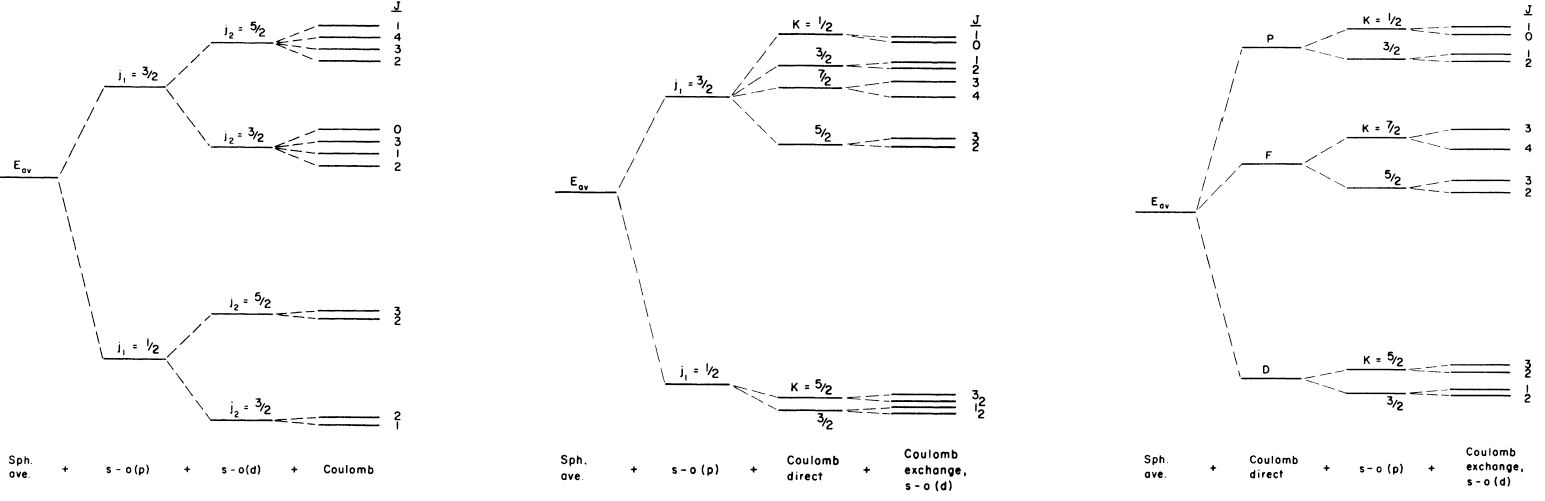
\includegraphics[scale=0.4]{ch1/image12}
	\captionof{figure}{Couplage $jj$ (gauche), $JK$ (centre) et $LK$ (droite)}
\end{center}

On peut comme précédemment passer d'une base à une autre. Pour quatre moments angulaires,
les matrice de changement de bases les plus compliquées sont proportionnelles aux symboles
$9j$. Pourquoi ce nom ? Car on a 9 moments angulaires : par exemple; 4 au départ, 
2 intermédiaires pour $LS$, deux pour $jj$ et le résultat $J$. Pour le passage $LS\leftrightarrow
jj$, nous avons
\begin{equation}
T_{LS,jj} = [L,S,j_1,j_2]^{1/2}
\left\{ \begin{array}{ccc}
l_1  & l_2 & L \\ s_1 & s_2 & S \\
j_1 & j_2 & J \end{array} 
\right\}
\end{equation}
où les $9j$ doivent satisfaire six règles triangulaires
\begin{equation}
\delta(l_1 l_2  L) , 
\delta(s_1 s_2  S) ,
\delta(L S J),
\delta(l_1 s_1 j_1) ,
\delta(l_2 s_2  j_2) ,
\delta(j_1 j_2  J)
\end{equation}
Parfois, les matrices de changement de base peuvent être plus simple car il existe
certaines règles sélectives. Par exemple, si $K=K'$, on n'aura plus que quatre règles
triangulaires à respecter
\begin{equation}
T_{LK',j_1 K} = 
{\color{red} \delta_{K,K'}}
(-1)^{l_2 + s_1 +L + j_1} 
[L, j_1]^{1/2}
\left\{ \begin{array}{ccc}
l_2  & l_1 & L \\ s_1 & K & j_1  \end{array} 
\right\}
\end{equation}
Pour l'élaboration des matrices de recouplages (\textit{slide 61-64}), voir notes du
cours 4. Certaines matrices sont plus difficile à obtenir que d'autres (par exemple,
$LS-jj$), mais on peut s'en sortir en faisant des produits de matrices. Ces matrices
sont intéressantes car elles peuvent être lues dans les deux sens.

\begin{itemize}
\item[$\bullet$] Horizontalement ; passage de $LSJ$ à $jj'J$, soit $ \vert LS J \rangle =
 \sum_{ j j' } \vert jj'J \rangle
\langle jj'J
 \vert LS J \rangle$. On trouve
 \begin{equation}
  \vert \; ^1P_1 \rangle =
\frac{1}{3} \sqrt{5}  \; 
\vert \left(
  \frac{3}{2}  \frac{3}{2} \right)_1 \rangle
+
\frac{1}{3}  \; 
\vert \left(
  \frac{3}{2}  \frac{1}{2} \right)_1 \rangle
-
\frac{1}{3}  \; 
\vert \left(
  \frac{1}{2}  \frac{3}{2} \right)_1 \rangle
+
\frac{1}{3} \sqrt{2}  \; 
\vert \left(
  \frac{1}{2}  \frac{1}{2} \right)_1 \rangle
 \end{equation}
\item[$\bullet$] Verticalement ; pour la \textbf{transformation inverse}, soit 
$ \vert jj' J \rangle =
 \sum_{ LS } \vert LSJ \rangle
\langle LSJ
 \vert jj' J \rangle$. On trouve
 \begin{equation}
 \vert \left(
  \frac{3}{2}  \frac{1}{2} \right)_1 \rangle
=
-\frac{1}{3} \sqrt{\frac{5}{6}}  \; 
\vert \; ^3D_1 \rangle 
+
\frac{1}{\sqrt{2}}  \; 
\vert \; ^3P_1 \rangle 
+
\frac{1}{3}  \; 
\vert \; ^1P_1 \rangle 
-
\frac{2}{3} \sqrt{\frac{2}{3}}  \; 
\vert \; ^3S_1 \rangle
 \end{equation}
\end{itemize}
On peut montrer que nous avons bien la transformation inverse pour une lecture
verticale. Nous avons d'une part
\begin{equation}
 \vert LS J \rangle =
 \sum_{ j j' } \vert jj'J \rangle
\langle jj'J  \vert LS J \rangle 
=
 \sum_{ j j' } \vert jj'J \rangle T_{LS,jj'}
\end{equation}
$\mbox{avec}~  T_{LS,jj'} = \langle jj'J  \vert LS J \rangle$, et d'autre part
\begin{equation}
 \vert jj' J \rangle =
 \sum_{ LS } \vert LSJ \rangle
\langle LSJ
 \vert jj' J \rangle
= 
\sum_{ LS } \vert LSJ \rangle
U_{jj',LS}
\end{equation} 
$\mbox{avec}~  U_{jj',LS} = \langle LSJ  \vert jj'J\rangle$. La transformation 
étant \textbf{unitaire}, on a 
\begin{equation}
U = T^{-1} = T^{\dagger} 
\rightarrow
U_{jj',LS} = \langle LSJ  \vert jj'J\rangle 
= \left( T_{LS,jj'} \right)^\ast
= \left( \langle jj'J  \vert LSJ \rangle \right) ^\ast
\end{equation}
De plus, les matrices de transformations sont \textbf{réelles} (orthogonales)
\begin{equation}
U_{jj',LS} = \langle LSJ  \vert jj'J\rangle 
=  T_{LS,jj'} 
=  \langle jj'J  \vert LSJ \rangle
\end{equation}
On montre ainsi le résultat attendu
\begin{equation}
 \vert jj' J \rangle =
 \sum_{ LS } \vert LSJ \rangle
\langle jj' J  \vert LSJ  \rangle
~~ \mbox{et} ~~
 \vert LS J \rangle =
 \sum_{ j j' } \vert jj'J \rangle
\langle LSJ   \vert  jj'J \rangle
\end{equation}\ \\

Comme annoncé, une \textbf{séquence} de recouplages peut être représenté
par un produit matriciel. On peut alors écrire quelque chose de compliqué
comme un produit de matrices "simples"
\begin{equation}
{\bf T}_{ {\color{blue} LS} \mbox{-} {\color{red} jj'} } =
{\bf T}_{ {\color{blue} LS} \mbox{-}  LK }
{\bf T}_{ LK \mbox{-}  jK }
{\bf T}_{ jK \mbox {-}  {\color{red} jj'} }
\end{equation}

\subsection{Passage de $pp'$ à $p^2$}
Lorsqu'on étudie le cas des électrons équivalents, il ne faut pas oublier que
\textsc{Pauli} rentre en action. Pour le couplage de deux électrons, il était
nécessaire que $(L+S)$ soit pair pour que la fonction ne s'annule pas. Comment
transposer cette condition quand on travaille avec $j$? Regardons l'opérateur de 
permutation
\begin{equation}
P_{12}\ket{j_1j_2'JM} = \ket{j_2j_1'JM}
\end{equation}
$P_{12}$ n'est pas fonction propre, car il ne s'agit pas du même \textit{ket}. Par
contre, on a bien $[P_{12},H]=0$ car les particules sont indiscernables. Appliquons
$P_{12}$ sur l'état suivant
\begin{equation}
P_{12}\left\{\frac{1}{\sqrt{2}}\alpha\ket{j_1j_2'JM}+\beta\ket{j_2j_1'JM}\right\} =
\pm \left\{\dfrac{1}{\sqrt{2}}\dots\right\}
\end{equation}
Comme nous avons des fermions, il nous faut une fonction antisymétrique par rapport à
l'échange. On prend alors le signe négatif pour créer une fonction antisymétrique par
rapport à l'échange. Si les électrons sont équivalents :
\begin{equation}
\begin{array}{ll}
P_{12}\left\{\frac{1}{\sqrt{2}}\alpha\ket{j_1j_2'JM}+\beta\ket{j_2j_1'JM}\right\} &=\DS\frac{1}{\sqrt{2}}
\left[\ket{j_1j_2JM}-(-1)^{j+j-J}\ket{j_1j_2JM}\right]\vspace{2mm}\\
&=\DS \frac{1}{\sqrt{2}}\ket{j_1j_2JM}\left[1-(-1)^{j+j-J}\right]
\end{array}
\end{equation}
Pour éviter l'annulation, il faut que $J$ soit pair. Lorsque les électrons sont
équivalents, nous avons une réduction du nombres d'états possibles 
\begin{center}
	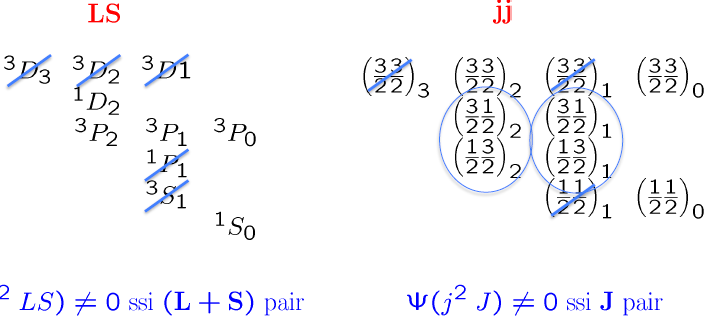
\includegraphics[scale=0.5]{ch1/image13}
	\captionof{figure}{ }
\end{center}
De plus, les états qui sont dans les cercles vont fusionner car ils sont indiscernables. 
Ainsi, pour deux électrons équivalents ($p^2$), les deux états $(3/2,1/2)$ et $(1/2,3/2$ sont
dits \textbf{coalescent}. Les matrices de recouplage (voir \textit{slide 71-72} sont ainsi
fortement réduites grâce à l'annulation de certaines fonctions.

\section{Antisymétrisation et parenté fractionnelle}

	\begin{wrapfigure}[11]{r}{3cm}
	\vspace{-5mm}
	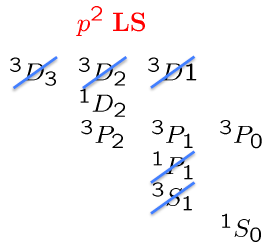
\includegraphics[scale=0.5]{ch1/image14}
	\captionof{figure}{ }
	\end{wrapfigure}
	
\subsection{Configuration $p^3$}	
Nous connaissons la configuration $p^2$ dans le couplage $LS$ : il était nécessaire que
$(L+S)$ soit un nombre pair pour que la fonction d'onde de l'état ne s'annule pas\footnote{Voir
notes slide 73 pour un exemple sur le traitement des électrons $d^2$ et $dd'$.} L'idée ici est
de créer $p^3$ à partir de $p^2$, c'est à dire
\begin{equation}
{\color{red}  p^2
\stackrel{+p}{\longrightarrow}
p^3 ~?? }
\end{equation}
La question que l'on se pose est \textit{dans quel cas cette fonction va survivre}
\begin{equation}
{\color{blue} \Psi (l^3 \; L'S') \ne 0 ~\mbox{ssi~??}  }
\end{equation}

Nous avons six moments angulaires
\begin{equation}
{\bf l_1} = {\bf l_2} =  {\bf l_3} =  {\bf 1},\qquad\qquad
{\bf s_1} = {\bf s_2} = {\bf s_3} = {\bf 1/2} 
\end{equation}
Nous pouvons avoir trois configurations possibles, en fonction du nombre d'électrons 
équivalents (ce qui change radicalement le nombre de lignes dans le sudoku)
\begin{enumerate}
\item Configuration $pp'p''$
\begin{equation}
g (pp'p'') = \left( \frac{6!}{1! (6-1)!} \right)^3 = 6^3 = 216
\end{equation}
\item Configuration $p^2p'$
\begin{equation}
g (p^2 p') = \left( \frac{6!}{2! (6-2)!} \right)
\left( \frac{6!}{1! (6-1)!} \right) = 15 \times 6 = 90
\end{equation}
\item Configuration $p^3$
\begin{equation}
g (p^3) = \frac{6!}{3! (6-3)!} = 20
\end{equation}
\end{enumerate}
On s'intéresse ici à la troisième configuration (mettre trois particules dans six boîtes). 
Pour connaître les états possibles ($^4S, ^2D$ et $^2P$), il est nécessaire de faire un
sudoku, les électrons étant équivalents (voir \textit{slide 75}).\\

Reprenons le coefficient de recouplage que nous avions introduit à la \textsc{Section 4}
(\textit{slide 20}) pour le couplage de \textbf{trois} moments angulaires (qui fait intervenir
un coefficient $6j$) :
\begin{equation}
\langle [ (j_1 j_2) J', j_3] JM 
\vert [j_1,(j_2 j_3) J''] JM \rangle
= 
(-1)^{j_1+j_2+j_3+J} [J',J'']^{1/2} \left\{ 
\begin{array}{ccc}
j_1 & j_2 & J' \\
j_3 & J & J''
\end{array} \right\}
\end{equation}
Nous avons deux histoires : celle de l'électron 1 et 2 que nous identifions avec une barre
et une seconde tandis celle de l'électron 2 et 3 sont identifiée avec des \textit{prim}. Ici, $LS$ désigne trois électrons mais $\overline{LS}$
ne concerne que les deux premiers. Regardons pour ces deux premiers électrons
\begin{equation}
\vert l^2 \overline{LS } \rangle
=  \vert l(1) l(2) \overline{LS} \rangle 
\frac{1}{2} 
\left\{ 1 
+ (-1)^{2l-\overline{L}-\overline{S}} 
 \right\} = \vert l(1) l(2) \overline{LS} \rangle 
~~\mbox{si}~~
(\overline{L}+\overline{S})~\mbox{est pair}
\end{equation}
Nous couplons ici deux moments angulaires : le premier dans $l(1)$ et le second également, $l(2)$. 
Cette fonction d'onde doit être antisymétrique à l'échange et résister à \textsc{Pauli} : un 
terme de phase va apparaître. Seuls les états ou $(\bar{L}+\bar{S})$  impairs vont subsister.\\

Couplons maintenant ces deux électrons avec le troisième pour former $LS$
\begin{equation}
\begin{array}{l}
\DS\vert \left( l^{2} \; \overline{L} \overline{S}, l (3) \right) 
L S \rangle 
= (-1)^{3l +L +3s +S} [ \overline{L} , \overline{S} ]^{1/2}\vspace{2mm}\\ \DS
\qquad\qquad\qquad\qquad\qquad\times  \sum_{L' S'} [ L', S' ]^{1/2} 
\left\{ 
\begin{array}{ccc}
l & l & \overline{L} \\
l & L & L'
\end{array}
\right\}
\left\{ 
\begin{array}{ccc}
s & s & \overline{S} \\
s & S & S'
\end{array}
\right\}
\vert \left( l(1), l(2) l(3)  L' S' \right) L S \rangle
\end{array}
\end{equation}
Lisons le premier $6j$. Nous couplons ici $ll$ à $l$. Les $l^2$ donnent naissance à un $\bar L$.
Ensuite, on vient ajouter un troisième moment angulaire $l$ (bas à gauche) que l'on couple
avec $\bar L$. Les autres règles triangulaires nous donnent quatre vertex et chacune nous rappelle
ce qui s'est passé. Regardons le \textit{ket} à droite. On voit $l(1)$ séparé et $l(2)$ de la
deuxième paire est couplé avec $l(3)$ pour donné $L'S'$, puis nous avons le $LS$ final. On 
fait de même pour le spin. Qu'est ce qui s'est passé pour avoir cette égalité ? Cela fait penser à un
 couplage de trois moments
angulaires. \\

Pour contruire ce dernier état, nous avons du sommer sur tous les $L'S'$. Cette sommation 
contient donc des termes $(L'+S')$ \textbf{impairs} et ne peut être antisymétrique à l'échange
par rapport à $(2)$ et $(3)$ ! A priori, elle n'est donc \textbf{pas} antisymétrique ! Reprenons
le terme de couplage
\begin{equation}
\begin{array}{l}
\DS{\color{blue}\vert \left( l^{2} \; \overline{L} \overline{S}, l (3) \right) 
L S \rangle }
= (-1)^{3l +L +3s +S} [ \overline{L} , \overline{S} ]^{1/2}\vspace{2mm}\\ \DS
\qquad\qquad\qquad\qquad\qquad\times  \sum_{L' S'} [ L', S' ]^{1/2} 
\left\{ 
\begin{array}{ccc}
l & l & \overline{L} \\
l & L & L'
\end{array}
\right\}
\left\{ 
\begin{array}{ccc}
s & s & \overline{S} \\
s & S & S'
\end{array}
\right\}
\vert \left( l(1), l(2) l(3)  L' S' \right) L S \rangle
\end{array}
\end{equation}
Nous allons être embêté car certains termes sont impossibles. Par contre, on peut toujours
envisager une combinaison linéaire de ces objets bleus, en sommant sur $\overline{LS}$, où 
les termes qui polluent l'histoire disparaissent
\begin{equation}
 \vert l^3 \alpha LS \rangle =
 \sum_{ \overline{L} \overline{S}  } 
 {\color{blue}
\vert ( l^{2} \; \overline{L} \overline{S}, l (3) )
L S \rangle }
\; 
 {\color{red}( } l^{2}  \overline{L} \overline{S} 
{\color{red} \vert \} }
 l^3 \alpha LS {\color{red} )} \; , 
\hspace*{0.5cm} 
(\overline{L} + \overline{S}) ~\mbox{pair}
\label{eq:c}
\end{equation}
L'idée est de "venir avec l'indice 3 sans antisymétriser" et de considérer la bonne combili
afin d'avoir une fonction antisymétrique à l'échange (1-2, 2-1 et 2-3). Ceci est l'état que nous recherchons, à savoir l'état permis pour trois électrons équivalents 
dans $l$. Nous l'avons ici exprimer comme une sommes des termes vus précédemment mais avec des
coefficients (rouge) tels qu'ils éliminent les contributions $(L'+S')$ impair. Sous ces conditions, nous avons la fonction d'onde décrivant trois fermions qui n'est pas 
décrite par des états polluants. \\

Dans la dernière \textbf{combinaison linéaire}, les coefficients ${\color{red}(|\})}$ sont tels que
\textbf{toutes} les fonctions
\begin{equation}
\vert \left( l(1), l(2) l(3)  L' S' \right) L S \rangle
\end{equation}
avec $(L'+S')$ impair \textbf{disparaissent}. Ainsi, la fonction d'onde $\ket{l^3\alpha LS}$ sera
\textbf{antisymétrique} pour $(1,2)$ et $(2,3)$. Elle le sera donc aussi pour $(1,3)$ et heureusement
car nous l'avons construite pour ça. On peut enfin comprendre le titre de la section : les 
\textit{parents} viennent de la génération précédente. Dans un système à $n$ particules, on se
réfère à $(n-1)$ et on ajoute la $n^e$ particule. La génération précédente est ici le 
$\overline{LS}$ (bleu) que l'on va pondérer par les coefficients rouges qui ont la propriété
remarquable d'éliminer ce que l'on ne veut pas. On va ainsi construire $p(3)$ à partir de 
$p(2)$\footnote{On construit un état à trois particules en prenant un état permis de la génération précédente (papa, maman) et on va lui mettre le bout manquant pour créer l'état à 3 particules.}, $d(5)$ à partir de $d(4)$, etc. C'est comme ceci que l'on construit des fonctions 
antisymétriques par rapport à l'échange.\\

En résumé
\begin{itemize}
\item[$\bullet$] Le terme $LS$ qui en découle sera un terme permis pour $l^3$
\item[$\bullet$] Les termes $\bar{LS}$ sont les termes \textbf{parents}
\item[$\bullet$] Les coefficients ${\color{red}(|\})}$ sont appelés \textbf{coefficient de 
parenté fractionnelle} (cfp)
\end{itemize}

\subsection{Application à la configuration $p^3$ (exercice)}
\subsubsection{Premier exercice}
Nous allons ici prendre $p^2$ comme parent pour $p^3$. Regardons ce que peut donner les 
deux états
\begin{equation}
p^2 \Rightarrow\ ^1S, ^1D, 3^P,\qquad\qquad\qquad
p^3 \Rightarrow\ ^4S, ^2D, 2^P,\qquad\qquad\qquad
\end{equation}
Nous voulons coupler 1-2 puis recombiner le résultat avec 3. Particularisons à notre exercice
\begin{equation}
\begin{array}{l}
\DS  {\color{blue}
\vert \left( p^{2} \; \overline{L} \overline{S}, p \right) L S 
\rangle  }
= (-1)^{s +L  +S} [ \overline{L} , \overline{S} ]^{1/2}\vspace{2mm}\\
\qquad\qquad\qquad\qquad\qquad\DS \times  \sum_{L' S'} [ L', S' ]^{1/2} 
\left\{ 
\begin{array}{ccc}
1 & 1 & \overline{L} \\
1 & L & L'
\end{array}
\right\}
\left\{ 
\begin{array}{ccc}
\frac{1}{2} & \frac{1}{2} & \overline{S} \\
\frac{1}{2} & S & S'
\end{array}
\right\}
\vert \left( p, pp  L' S' \right) L S \rangle
\end{array}
\end{equation}
Supposons que l'on veut \textbf{créer} un état ${\color{red} S=3/2}$, soit un état quadruplet
à trois électrons (on verra plus tard qu'il faut $L=0$ (on peut déjà le voir ci-dessus, dans les
états de $p^3$)). Pour avoir $S=3/2$, il faut trois spins \textit{up}. Nous allons rajouter un
$up$ à \textit{up-up}. Or, un état \textit{up-up} n'est possible que pour un état triplet. Regardons
les états "proposés" par le parent $p^2$. Il possède un (et un seul) état triplet,\ $^3P$. C'est
nécessairement le parent
\begin{equation}
 p^{2} \; \overline{L} \overline{S} = p^2 \; ^3P
\end{equation}
Il faut donc que $\bar S = S' = 1$. Nous devons également avoir $L=1=P$ (c'est aussi le
seul disponible par le parent). Comme c'est le seul parent "permis", il va être pondéré d'un 
coefficient 1 : ce sera son seul cfp non nul ! L'expression \eqref{eq:c} devient
\begin{equation}
\ket{p^3\alpha LS} = \sum_{\overline{LS}} \ket{l^2\overline{LS},l(3)\alpha LS}(l^2\overline{LS}|
l^3\alpha LS)
\end{equation}
Dans notre cas, on s'intéresse à $L=0$
\begin{equation}
\ket{p^3\ ^4S} =1.\ket{p^2\ ^3P,p(S)\ ^4S}  + 0. \ket{p^2\ ^1S,p(3)\ ^4S} + 0.\ket{p^2\ ^1D,p(3)\ 
^4S}
\end{equation}
On peut retrouver ceci de façon "plus analytique" :
\begin{equation}
\begin{array}{ll}
 {\color{blue}
\vert \left( p^{2} \; \; ^3P, p \right) \; ^4 L^o \rangle  }
 &\DS= (-1)^{L} \cdot 3 \sum_{L'} (3[ L'])^{1/2} 
\left\{ 
\begin{array}{ccc}
1 & 1 & 1 \\
1 & L & L'
\end{array}
\right\}
\left\{ 
\begin{array}{ccc}
\frac{1}{2} & \frac{1}{2} & 1 \\
\frac{1}{2} & \frac{3}{2} & 1
\end{array}
\right\}
\vert \left( p, pp  \; ^3L' \right) \; ^4L^o \rangle\vspace{2mm}\\
&\DS =
(-1)^{L+1 } \sum_{L'} (3[ L'])^{1/2} 
\left\{ 
\begin{array}{ccc}
1 & 1 & 1 \\
1 & L & L'
\end{array}
\right\}
\vert \left( p, pp  \; ^3L' \right) \; ^4L^o \rangle
\end{array}
\end{equation}
Si ${\color{red} L=0}$, le seul $L'$ permis est $L'=1$
\begin{equation}
\left\{ 
\begin{array}{ccc}
1 & 1 & 1 \\
1 & 0  & L'
\end{array}
\right\}
\propto \delta_{L',1}
\end{equation}
Ainsi, la somme sur $L'$ se réduit à un seul terme
\begin{equation}
 {\color{blue}
\vert \left( p^{2} \; \; ^3P, p \right)  }\;  {\color{red}^4 S^o}
 \rangle 
= -3 
\left\{ 
\begin{array}{ccc}
1 & 1 & 1 \\
1 & 0 & 1
\end{array}
\right\}
\vert \left( p, pp  \; ^3P \right) \; ^4S^o \rangle  
= \vert \left( p, pp  \; ^3P \right) \; ^4S^o \rangle
\end{equation}
Le terme en bleu était déjà antisymétrique. Maintenant, nous avons l'antisymétrie par rapport
à 2-3 : cette fonction est donc antisymétrique par rapport à tout. La seule façon de faire est
que ce coefficient vaut 1 : comme il n'y a pas autre chose que le $^3P$, c'est le seul coefficient
qui vaut 1. \\

Dès lors, cet état est acceptable car $(L'+S')$ est pair. Ce terme existe et le cfp correspondant
vaut
\begin{equation}
\begin{array}{c}
  {\color{red}( } p^{2}  \overline{L} \overline{S} 
{\color{red} \vert \} }
 p^3 \; ^4S {\color{red} )} = 1 ~\mbox{pour}~
\overline{L} \overline{S}  = \; ^3P\\
  {\color{red}( } p^{2}  \overline{L} \overline{S} 
{\color{red} \vert \} }
 p^3 \; ^4S {\color{red} )} = 0 ~\mbox{pour}~
\overline{L} \overline{S}  = \; ^1D\\
  {\color{red}( } p^{2}  \overline{L} \overline{S} 
{\color{red} \vert \} }
 p^3 \; ^4S {\color{red} )} = 0 ~\mbox{pour}~
\overline{L} \overline{S}  = \; ^1S
\end{array}
\end{equation}
C'est bien ce que nous avions annoncé précédemment! On pondère de 1 le terme antisymétrique
par rapport à l'échange, il n'y a rien à faire. C'est ici la \textbf{seule} façon de construire
un tel état : on part du $\ ^3P$ et on n'aura pas de souci pour construire le suivant. 

\subsubsection{Second exercice}
Essayons de construire le quadruplet $D$. Si l'on fait le sudoku, on se rend compte que cet état
n'existe pas, mais essayons tout de même. Exprimons le couplage
\begin{equation}
\begin{array}{ll}
 {\color{blue}
\vert \left( p^{2} \; \; ^3P, p \right)  }\;  {\color{red}^4 D^o}
 \rangle 
&\DS= 
 - 3 
\left\{ 
\begin{array}{ccc}
1 & 1 & 1 \\
1 & 2 & 1
\end{array}
\right\}
\vert \left( p, pp  \; ^3P \right) \; ^4D^o \rangle 
- \sqrt{15}
\left\{ 
\begin{array}{ccc}
1 & 1 & 1 \\
1 & 2 & 2
\end{array}
\right\}
\vert \left( p, pp  \; ^3D \right) \; ^4D^o \rangle\\
&\DS=
- \frac{1}{2}  
\vert \left( p, pp  \; ^3P \right) \; ^4D^o \rangle 
+ \frac{\sqrt{3}}{2} \; 
\vert \left( p, {\color{red} pp  \; ^3D} \right) \; ^4D^o \rangle
\end{array}
\end{equation}
En exprimant le couplage, on voit l'apparition d'une pollution : un terme interdit pour 
${\color{red}pp\ ^3D}$. Celui-ci n'est pas antisymétrique pour l'échange 2-3 car $(L+S)$ est impair. Ceci
démontre qu'il est impossible de construire un terme $\ ^4D$ découlant de $p^3$ antisymétrique
pour 1-2 et 2-3. Comme ce quadruplet est impossible, les trois cpf sont forcément nuls
\begin{equation}
\begin{array}{c}
  {\color{red}( } p^{2}  \overline{L} \overline{S} 
{\color{red} \vert \} }
 p^3 \; ^4D {\color{red} )} = 0 ~\mbox{pour}~
\overline{L} \overline{S}  = \; ^3P\\
  {\color{red}( } p^{2}  \overline{L} \overline{S} 
{\color{red} \vert \} }
 p^3 \; ^4D {\color{red} )} = 0 ~\mbox{pour}~
\overline{L} \overline{S}  = \; ^1D\\
  {\color{red}( } p^{2}  \overline{L} \overline{S} 
{\color{red} \vert \} }
 p^3 \; ^4D {\color{red} )} = 0 ~\mbox{pour}~
\overline{L} \overline{S}  = \; ^1S
\end{array}
\end{equation}

\subsubsection{Élimination des contributions symétriques}
Illustrions l'utilisation des cfp pour éliminer les contributions non antisymétriques. Considérons
le terme $^2D$ construit à partir du parent $^3P$
\begin{equation}
\begin{array}{l}
\DS {\color{blue}
\vert \left( p^{2} \; \; {\color{magenta} ^3P}, p \right)  }
\;  {\color{red} ^2D^o}
 \rangle 
= 
- \frac{\sqrt{3}}{4} \; 
\vert \left( p, {\color{red} pp  \; ^1P } \right) \; ^2D^o \rangle
 - \frac{1}{4}  
\vert \left( p, pp  \; ^1D \right) \; ^2D^o \rangle\vspace{2mm}\\ \DS
\qquad\qquad\qquad\qquad\quad+ \frac{3}{4}  
\vert \left( p, pp  \; ^3P \right) \; ^2D^o \rangle 
+ \frac{\sqrt{3}}{4} \; 
\vert \left( p, {\color{red} pp  \; ^3D } \right) \; ^2D^o \rangle 
\end{array}
\end{equation}
Cette fonction est inacceptable pour trois fermions car elle n'est pas antisymétrique
par rapport à (23). Il existe un autre parent ($\ ^1D$) à partir duquel le terme $^2D$ peut être
formé
\begin{equation}
\begin{array}{l}
\DS{\color{blue}
\vert \left( p^{2} \; \; {\color{magenta} ^1D}, p \right)  }\;  {\color{red} ^2D^o}
 \rangle 
= 
- \frac{\sqrt{3}}{4} \; 
\vert \left( p, {\color{red} pp  \; ^1P}  \right) \; ^2D^o \rangle
 + \frac{3}{4}  
\vert \left( p, pp  \; ^1D \right) \; ^2D^o \rangle\vspace{2mm}\\
\DS\qquad\qquad\qquad\qquad\quad - \frac{1}{4}  
\vert \left( p, pp  \; ^3P \right) \; ^2D^o \rangle 
+ \frac{\sqrt{3}}{4} \; 
\vert \left( p, { \color{red} pp  \; ^3D } \right) \; ^2D^o \rangle
\end{array}
\end{equation}
Cette seconde fonction est tout aussi inacceptable. \textbf{Par contre}, on peut toujours combiner
ces deux fonctions 
\begin{equation}
\alpha  {\color{blue}
\vert \left( p^{2} \; \; {\color{magenta} ^3P}, p \right)  }
\;  {\color{red} ^2D^o}
 \rangle 
+ \beta {\color{blue}
\vert \left( p^{2} \; \; {\color{magenta} ^1D}, p \right)  }
\;  {\color{red} ^2D^o}
 \rangle
\end{equation}
Et choisir judicieusement $(\alpha,\beta)$ pour éliminer les contributions indésirables, qui ne
sont pas antisymétriques pour $(23)$. Ainsi, la combinaison
\begin{equation}
\vert p^3 \; ^2D \rangle =
\frac{1}{\sqrt{2}}  {\color{blue}
\vert \left( p^{2} \; \; {\color{magenta} ^3P}, p \right)  }
\;  {\color{red} ^2D^o}
 \rangle 
- \frac{1}{\sqrt{2}}
 {\color{blue}
\vert \left( p^{2} \; \; {\color{magenta} ^1D}, p \right)  }
\;  {\color{red} ^2D^o}
 \rangle
\end{equation}
est la clé pour restaurer l'antisymétrie complète de la fonction $p^3$. Ce faisant, nous
avons déterminer les trois cpf :
\begin{equation}
\begin{array}{c}
  {\color{red}( } p^{2}  \overline{L} \overline{S} 
{\color{red} \vert \} }
 p^3 \; ^2D {\color{red} )} = +1/\sqrt{2} ~\mbox{pour}~
\overline{L} \overline{S}  = \; ^3P\\
  {\color{red}( } p^{2}  \overline{L} \overline{S} 
{\color{red} \vert \} }
 p^3 \; ^2D {\color{red} )} = -1/\sqrt{2} ~\mbox{pour}~
\overline{L} \overline{S}  = \; ^1D\\
  {\color{red}( } p^{2}  \overline{L} \overline{S} 
{\color{red} \vert \} }
 p^3 \; ^2D {\color{red} )} = 0 ~\mbox{pour}~
\overline{L} \overline{S}  = \; ^1S
\end{array}
\end{equation}
On peut montrer de façon similaire que
\begin{equation}
\vert p^3 \; ^2P^o \rangle =
+ \frac{2}{\sqrt{18}}   {\color{blue}
\vert \left( p^{2} \; \; {\color{magenta} ^1S}, p \right)  }
\;  {\color{red} ^2P^o}
 \rangle 
- \frac{3}{\sqrt{18}}
 {\color{blue}
\vert \left( p^{2} \; \; {\color{magenta} ^3P}, p \right)  }
\;  {\color{red} ^2P^o}
 \rangle 
- \sqrt{\frac{5}{18}} 
 {\color{blue}
\vert \left( p^{2} \; \;
{\color{magenta} ^1D }, p \right)  }
\;  {\color{red} ^2P^o}
\end{equation}
Un tableau reprenant les cpf est repris au \textit{slide 85}. Voir notes manuscrites à partir
du \textit{slide 83} pour le calcul de coefficients (exercice fait en cours) (\textbf{à refaire, pas évident!}).



\section{Couplages et recouplages de $n$ moments angulaires}
\subsection{Symboles $3(n-1)-j$}
Ce que nous avons fait peut être étendu pour définir les symbole $3(n-1)-j$.
$$\begin{array}{ll}
2~\mbox{moments angulaires}  &   
\rightarrow \mbox{symboles}~3\mbox{-}j \\
3~\mbox{moments angulaires}  &   
\rightarrow  \mbox{symboles}~6\mbox{-}j \\
4~\mbox{moments angulaires}  &   
\rightarrow \mbox{symboles}~9\mbox{-}j \\
5~\mbox{moments angulaires}  &   
\rightarrow \mbox{symboles}~12\mbox{-}j\\
\ldots & \ldots \\
{\color{red} n} ~\mbox{moments angulaires}  &   
\rightarrow  \mbox{symboles}~{\color{red} 3(n-1)\mbox{-}j  }
\end{array}$$

\subsection{Algèbre graphique}
\subsubsection{Trois moments angulaires}
On peut dessiner le recouvrement entre l'arbre de couplage d'un schéma et l'arbre de 
couplage d'un autre schéma. 
\begin{center}
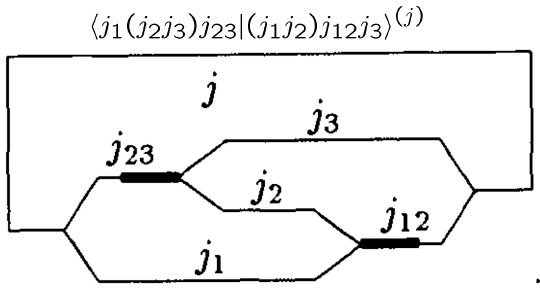
\includegraphics[scale=0.5]{ch1/image15}
\captionof{figure}{Nous avons une histoire de couplage "vers la gauche" et une autre "vers la droite".}
\end{center}
On peut procéder de la sorte pour quatre moments angulaire (voir \textit{slide 88}).

\section{Arbre de couplages pour un atome}
Considérons la \textbf{configuration électronique} d'un atome : $w_1$ électrons dans $n_1l_1$, 
etc : 
\begin{equation}
(n_1 l_1) ^{w_1} (n_2 l_2) ^{w_2} (n_3 l_3) ^{w_3}
\ldots
(n_x l_x) ^{w_x}  \ldots (n_m l_m) ^{w_m}
\end{equation}
avec $\sum_{i=1}^m w_i = N$. Nous allons coupler petit à petit les différentes couches
pour créer le \textbf{terme électronique}
\begin{equation}
\alpha  L S (M_L M_S)
\end{equation}
où $\alpha$ c'est toute l'histoire de $LS$ (soit la configuration électronique). Nous allons
ainsi créer pleins de niveaux qui ont chacun un $LS(M_LM_S)$ et une dégénérescence $G_{LS} = 
(2L+1)(2S+1)$.\\
\newpage

	\begin{wrapfigure}[15]{r}{8.5cm}
	%\vspace{-5mm}
	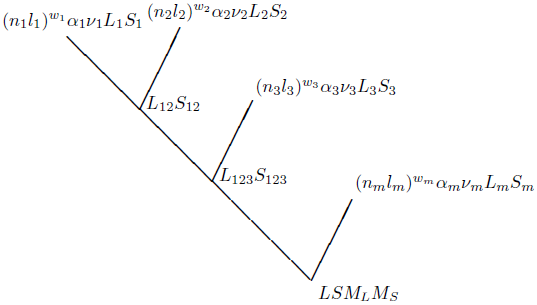
\includegraphics[scale=0.6]{ch1/image16}
	\captionof{figure}{ }
	\end{wrapfigure}
Nous allons ainsi créer l'\textbf{arbre de couplages} d'une CSF\footnote{Configuration State 
Function.}. Qu'est ce que $(n_1l_1)^{w_1}$ ? Pour caractériser $w_1$, on n'aura pas assez avec
$n_1$ et $w_1$ : il faut introduire d'autres nombres quantiques. On construit ainsi l'état à 
$N$ corps en construisant pas à pas les fonctions des différentes sous-couches. Pour cet arbre-ci,
on aura une série de triade de nombres quantiques (noté en rouge)

\begin{equation}
 m~ \mbox{``triades'' de couche}~
(n_x l_x) ^{w_x}  {\color{red} \alpha_x \nu_x L_x S_x }
\end{equation}
Nous avons bien
\begin{equation}
(2m-1) \mbox{``triades'' de nombres quantiques:}
\end{equation}
Avec $m$ triades  de couches et pleins de nombres quantiques intermédiaires : $L_{12}, S_{12}, 
L_{123}, S_{123},$ etc
\begin{equation}
(m-1)~ \mbox{nombres quantiques interm\'ediaires}
\end{equation}
J'ai noté "voir notes", mais je les trouves plus :D 

\section{Symétrie de couche, termes et séniorité}
\textit{J'ai un peu la flemme, cette dernière section sera principalement une retranscription
de mes notes}. Je fais référence à des notes que j'ai aussi perdues :D !\\

L'idée de ce tableau est de reprendre tout ce qu'on peut faire en satisfaisant \textsc{Pauli}.
Pour un électron $s$, j'ai deux boites $s$ et $\bar{s}$ et nous aurons l'un ou l'autre. C'est
forcément un doublet $S$. Pour deux électrons $s$, on peut avoir $s$ et $\bar s$ en même temps
et ainsi former le singlet $^1S$. Lorsqu'une couche est remplie c'est comme si elle était vide
car tous les nombres quantiques magnétiques se compensent. \\

Avoir 1 ou 5 électron(s) $p$, c'est la même chose. Il peut être doublet et seulement $P$ car il n'y
a qu'un $p$. Pour $p^2/p^4$, seul $(L+S)$ résistent  : on peut avoir un singlet $S$ ou un 
singlet $D$. Pour $p^3$, il faut faire un sudoku.\\

Pour les états $d$, même combat mais ici on voit que certains états portent le même nom  : $L$ et
$S$ \textbf{ne sont plus suffisant}. La colonne $g(nl^N)$ compte le nombre d'états qui ont la 
même symétrie $L$ et $S$, mais ceci n'est visiblement pas suffisant dans le couche $D$.\\

\begin{center}
La dégénérescence augmente rapidement avec $l$ et est d'autant plus grande que $N$ se rapproche de l'occupation de mi-couche\footnote{Aussi "voir notes", mais toujours perdues pfpfpfpf}
\end{center}
\begin{equation}
g(nl^N) = 
  \left( \begin{array}{cc}  2(2l+1) \\ N \end{array} \right) 
= \frac{[(2(2l+1)]!}{N![(2(2l+1)-N]!}
\end{equation}
De quel $^2D$ parlons nous dans $d^3$ ou $d^5$ ? On va devoir les différencier. Regardons 
d'abord pour un nombre d'électron impair
$$\begin{array}{c|ccccccc}
d^{\color{red} 1}    & ^2_{\color{red} 1}D   &      &      &      &      &  &\\
&&&&&&& \\
d^{\color{blue} 3}   &   ^2_{\color{red} 1}D    &
 ^2_{\color{blue} 3}D   &        & ^2_{\color{blue} 3}F  &  
 &  ^2_{\color{blue} 3}G & \\ 
&&&&&&&\\
d^5  &  ^2_{\color{red} 1}D     & ^2_{\color{blue} 3}D    &
 ^2_5D  & ^2_{\color{blue} 3}F & 
^2_5F & ^2_{\color{blue} 3}G  & ^2_5G  \\
&&&&&&&\\
\end{array}$$
Voir notes sur slides, plus facile par écrit pour voir qui vient de qui. En gros, on donne
une seigneurité la première voir qu'il apparaît (en bleu dans $d^3$, noir dans $d^5$ (ou on
attribue une seigneurité de 5 la première fois qu'il apparait et une de 3 pour dire qu'il vient
de $d^3$. Ce faisant on regarde les parents, mais également les grands-parents
\begin{equation}
d^q {\color{red} v}LS +d^2\ _0^1S \rightarrow
d^{q+1}{\color{red} v}LS
\end{equation}
Pour la couche $F$, on a énormément d'états. Même à l'aide des grands parents, on n'a pas assez
avec la seigneurité (trop de nouveaux avec le même nom)
$$\begin{array}{c|cccccccccccccc}
f^0   & ^1_0S  &&&&&&&&&& \\
&&&&&&&&&&& \\
f^{\color{red} 2}    & ^1_0S&  ^3_2P  & ^1_2D & {\color{red} ^3_2F} & ^1_2G &
^3_2H & ^1_2I & & & &  \\   
&&&&&&&&&&& \\
f^{\color{blue} 4}    & ^1_0S&  ^3_2P  & ^1_2D & {\color{red} ^3_2F} & ^1_2G & 
^3_2H & ^1_2I  & {\color{blue} ^3_4F}& 
 {\color{blue} ^3_4F}&  {\color{blue} ^3_4F}&
 \ldots \\
&&&&&&&&&&& \\
\end{array}$$
$$\mbox{La s\'eniorit\'e n'est pas suffisante} \rightarrow
(n_x l_x) ^{w_x}  {\color{red} \alpha_x \nu_ x } L_x S_x$$
 Le problème sera réglé en faisant l'usage
des groupes de \textsc{Lie} et en faisant intervernir le quasi-spin.

\begin{center}
Chaîne de groupes SO(7) $\supset$ G$_2$ $\supset$ SO(3)
\end{center}